% Smart Campus Classroom Management System — IEEE Technical Report
% SMU Mediterranean Institute of Technology | ISS Project 2025–2026
% Team: Ben Jemaa · Jallouli · Saadaoui · Ouertani · Day
%
% Compile sequence (Overleaf / local MiKTeX / TeX Live):
%   pdflatex main && bibtex main && pdflatex main && pdflatex main

\documentclass[journal]{IEEEtran}

%% ── Packages ──────────────────────────────────────────────────────────────
\usepackage[T1]{fontenc}
\usepackage[utf8]{inputenc}
\usepackage{graphicx}
\usepackage{hyperref}
\usepackage{booktabs}
\usepackage{listings}
\usepackage{xcolor}
\usepackage{amsmath}
\usepackage{float}
\usepackage{array}
\usepackage{tabularx}
\usepackage{multirow}
\usepackage{url}
\usepackage{cite}
\usepackage{microtype}

%% ── Graphics path ─────────────────────────────────────────────────────────
\graphicspath{{figures/}}

%% ── Hyperref setup ────────────────────────────────────────────────────────
\hypersetup{
  colorlinks = true,
  linkcolor  = blue!60!black,
  citecolor  = green!50!black,
  urlcolor   = blue!60!black,
  pdftitle   = {Smart Campus Classroom Management System},
  pdfauthor  = {SMU ISS Team 2025-2026},
}

%% ── Code listing style ────────────────────────────────────────────────────
\lstdefinestyle{pycode}{
  language     = Python,
  basicstyle   = \ttfamily\footnotesize,
  keywordstyle = \color{blue!70!black}\bfseries,
  commentstyle = \color{green!50!black}\itshape,
  stringstyle  = \color{red!60!black},
  breaklines   = true,
  frame        = single,
  numbers      = left,
  numberstyle  = \tiny\color{gray},
  xleftmargin  = 1.5em,
}

\lstdefinestyle{jsoncode}{
  basicstyle   = \ttfamily\footnotesize,
  breaklines   = true,
  frame        = single,
  numbers      = left,
  numberstyle  = \tiny\color{gray},
  xleftmargin  = 1.5em,
}

%% ── Title block ───────────────────────────────────────────────────────────
\title{Smart Campus Classroom Management System:\\
       An IoT and Edge-AI Approach to Automated Attendance,\\
       Environmental Monitoring, and At-Risk Detection}

\author{Mohamed~Hedi~Ben~Jemaa,~Ahmed~Amine~Jallouli,~Ali~Saadaoui,\\
        Abdelhamid~Ouertani,~and~Iyed~Day%
  \thanks{All authors are students at SMU\,--\,Mediterranean Institute of
    Technology, Tunis, Tunisia (ISS Project, Academic Year 2025\,--\,2026).
    Supervisor: SMU ISS Faculty.
    Manuscript submitted: May 2026.}}

%% ═══════════════════════════════════════════════════════════════════════════
\begin{document}

\maketitle

%% ── Abstract + Keywords ───────────────────────────────────────────────────
%% ── Abstract ──────────────────────────────────────────────────────────────
\begin{abstract}
This paper presents the design and implementation of the Smart Campus
Classroom Management System, an IoT and edge-AI platform developed at
SMU\,--\,Mediterranean Institute of Technology.  The system addresses
three core problems in traditional classroom operation: manual attendance
taking (up to 15~minutes per lecture), the absence of real-time
environmental monitoring, and the lack of early-warning mechanisms for
academically at-risk students.

The solution integrates an ESP32 microcontroller---equipped with
temperature, humidity, air-quality, and sound sensors---with a Raspberry
Pi~4B edge server that runs all services without cloud dependency.
Student attendance is automated via camera-based face recognition using
DeepFace/FaceNet 128-dimensional embeddings with cosine-distance
matching.  Sensor data is streamed over MQTT (Mosquitto broker) to a
FastAPI backend and forwarded in real time to a React professor dashboard
via WebSocket.  AC and lighting are controlled automatically based on
configurable thresholds, with manual professor override.  Attendance
records are synchronised to the Moodle LMS on session completion.

An AI analytics layer, built on a locally hosted Ollama phi3-mini LLM,
identifies at-risk students (below 70\% attendance) and generates
natural-language explanations; a deterministic forecasting pipeline
classifies per-course attendance trends and adds LLM-generated prose
interpretations.  The complete stack is containerised with Docker~Compose
and was delivered across 22 development phases within a single academic
semester.  Evaluation demonstrates full elimination of manual attendance
overhead, end-to-end sensor latency below 5~seconds, and AI pipeline
runtime reduction from approximately 14--16~minutes to 2--3~minutes
through batch-query optimisation.
\end{abstract}

%% ── Keywords ──────────────────────────────────────────────────────────────
\begin{IEEEkeywords}
IoT, smart classroom, face recognition, MQTT, FastAPI, edge computing,
LLM, at-risk detection, attendance automation, Raspberry Pi, ESP32,
Docker, WebSocket, Moodle
\end{IEEEkeywords}


%% ── Chapters ──────────────────────────────────────────────────────────────
%% ════════════════════════════════════════════════════════════════════════════
\section{Introduction}
\label{sec:intro}
%% ════════════════════════════════════════════════════════════════════════════

\subsection{Context and Motivation}
\label{subsec:context}

The growing adoption of Internet of Things (IoT) technology in education
has opened new possibilities for automating routine classroom tasks and
improving the quality of the learning environment.  Despite this trend,
many universities---including SMU\,--\,Mediterranean Institute of
Technology---continue to rely on manual processes for attendance
management and environmental control.  Professors spend up to 15~minutes
per lecture calling roll, consuming valuable instructional time.
Meanwhile, classroom HVAC systems and lighting are operated without any
sensor feedback, leaving occupant comfort dependent on manual judgment.
Early identification of students at risk of academic failure due to poor
attendance remains largely reactive, with intervention arriving after the
damage is already done.

The convergence of affordable edge hardware (ESP32, Raspberry Pi~4B),
open-source ML frameworks (DeepFace, Ollama), and lightweight message
protocols (MQTT) makes it feasible to deploy a fully autonomous
classroom management platform at minimal cost, running entirely on the
university's local area network with no cloud dependency.

\subsection{Problem Statement}
\label{subsec:problem}

Three concrete pain points motivate this work:

\begin{enumerate}
  \item \textbf{Attendance inefficiency.}  Manual roll-call consumes up
    to 15~minutes per session---time that reduces effective teaching time
    by 15--20\% for a 50-minute lecture.  Records are entered manually
    into the Moodle LMS, creating duplication of effort and data-entry
    errors.

  \item \textbf{Unmonitored environment.}  No real-time sensor data is
    available to inform HVAC or lighting decisions.  Temperature, humidity,
    CO$_2$/VOC levels, and occupancy are unknown to both professors and
    facility managers.

  \item \textbf{No early warning for at-risk students.}  Advising staff
    receive no automated signal when a student's attendance rate begins to
    decline.  Intervention is reactive rather than preventive, reducing
    its effectiveness.
\end{enumerate}

\subsection{Project Objectives}
\label{subsec:objectives}

The general objective of this project is to design and implement an
IoT-based smart classroom management system that automates student
attendance via camera-based face recognition, monitors classroom
environmental conditions in real time, enables automated and manual
control of AC and lighting, provides professors with a live web
dashboard, synchronises attendance to the Moodle LMS, and identifies
at-risk students and attendance trends using a locally hosted LLM---all
running on a Raspberry Pi~4B without cloud dependency.

The six specific objectives are:
\begin{enumerate}
  \item Automate student attendance recording using face recognition.
  \item Monitor classroom environmental conditions (temperature, humidity,
    air quality, sound) in real time.
  \item Enable automated and manual control of AC and lighting via relay
    actuation.
  \item Provide professors with a live web dashboard showing attendance,
    sensor data, and alerts.
  \item Synchronise attendance records to Moodle automatically on session
    end.
  \item Identify at-risk students and forecast attendance trends using AI
    analytics.
\end{enumerate}

\subsection{Scope and Limitations}
\label{subsec:scope}

The system is scoped to a single classroom room (\texttt{room1}) on the
university intranet.  All services run locally on the Raspberry Pi~4B;
there is no internet dependency during normal operation.  The academic
semester timeline constrained the project to a proof-of-concept
deployment with physical hardware; production hardening (HTTPS/WSS,
multi-room support) is identified as future work.

Hardware budget constraints led to the selection of the MQ-135 gas
sensor, whose output is uncalibrated and used comparatively rather than
as an absolute CO$_2$ reference.  The Raspberry Pi~4B's CPU limits
face-recognition throughput to 2~fps and phi3-mini inference to
10--30~seconds per student.

\subsection{Report Structure}
\label{subsec:structure}

Section~\ref{sec:literature} reviews related work on IoT-based attendance
systems, face recognition, and edge AI.
Section~\ref{sec:requirements} presents stakeholder analysis and
functional and non-functional requirements.
Section~\ref{sec:architecture} describes the full system architecture
across all subsystem layers.
Section~\ref{sec:implementation} details hardware assembly, firmware, and
software implementation.
Section~\ref{sec:ai} covers the AI analytics pipelines.
Section~\ref{sec:security} analyses security and privacy considerations.
Section~\ref{sec:testing} documents the testing and validation approach.
Section~\ref{sec:results} presents results and key lessons learned.
Section~\ref{sec:conclusion} concludes with a summary of contributions
and directions for future work.

%% ════════════════════════════════════════════════════════════════════════════
\section{Literature Review and Related Work}
\label{sec:literature}
%% ════════════════════════════════════════════════════════════════════════════

\subsection{Smart Classroom Systems: State of the Art}
\label{subsec:lit_smart}

Smart classroom systems have evolved significantly over the past decade
from simple RFID card readers to multi-sensor IoT platforms.  Early
approaches such as~\cite{rfid_attendance_2018} demonstrated that RFID
tags could replace paper registers, reducing attendance time to under
two minutes per lecture.  However, RFID systems require students to
actively tap a reader, introducing a proxy-attendance vulnerability and
necessitating additional hardware distributed to each student.

Subsequent work explored QR-code-based attendance~\cite{qr_attend_2020},
which requires only a smartphone but shares the proxy problem and depends
on stable Internet connectivity for code rotation.  Camera-based
approaches eliminate student action entirely: the system identifies
occupants passively, closing the proxy loophole and reducing
professor workload to zero for the attendance step.

A recurring limitation across these systems is the absence of an
integrated environmental monitoring layer and of any AI-driven academic
risk analysis.  They treat attendance as the sole data point, ignoring
classroom conditions that correlate with student engagement and comfort.

\subsection{Face Recognition in Attendance Systems}
\label{subsec:lit_face}

Face recognition for attendance has been studied extensively using
conventional CNN-based pipelines~\cite{facenet_2015, deepface_2021}.
FaceNet~\cite{facenet_2015} introduced the 128-dimensional embedding
space with triplet-loss training, enabling sub-centimetre face-to-face
distance computation via cosine similarity.  DeepFace~\cite{deepface_2021}
unifies multiple model backends (Facenet, ArcFace, VGG-Face) behind a
single Python API, significantly reducing integration effort.

Our system uses DeepFace with the Facenet backend.  Enrollment
generates a 128-dimensional float32 embedding averaged from up to five
reference images per student; recognition applies cosine-distance
thresholding ($d < 0.40$) at 2~fps.  This threshold is tighter than
the DeepFace default ($0.60$) to reduce false-positive attendance
records on a shared-CPU Raspberry Pi~4B.

Prior work~\cite{rpi_face_2022} showed that Facenet inference on an
RPi~4B reaches 1--3~fps under normal lighting, consistent with our
empirical observations.  The primary tradeoff is latency: the 2~fps
ceiling means a 30-student class requires up to 15~seconds to scan
all faces in one frame pass, motivating the snapshot-per-cycle
attendance model described in Section~\ref{subsec:recognition}.

\subsection{IoT Protocols for Educational Environments}
\label{subsec:lit_mqtt}

Three lightweight messaging protocols are commonly evaluated for IoT
sensor networks: MQTT~\cite{mqtt_spec_5}, CoAP~\cite{rfc7252_coap},
and HTTP polling.  MQTT's publish-subscribe architecture decouples
producers (ESP32 sensor nodes) from consumers (backend services)
without requiring the sensor to know the consumer's address.  Its
binary framing and persistent TCP connection produce less per-message
overhead than HTTP, and its broker-mediated delivery survives transient
client disconnections through configurable quality-of-service (QoS)
levels.

QoS~0 (fire-and-forget) is used throughout this system.  For sensor
readings published every 5~seconds, an occasional dropped message
causes at most a 10-second gap in the time-series record---acceptable
for environmental monitoring.  Upgrading to QoS~1 would guarantee
delivery at the cost of increased broker state and acknowledgement
round-trips, which is unnecessary on a local network with sub-1~ms
latency.

\subsection{Local LLM Inference at the Edge}
\label{subsec:lit_llm}

Recent advances in model quantisation have made it feasible to run
billion-parameter language models on commodity CPU hardware.  The
phi3-mini model~\cite{phi3_mini_2024} (3.8~B parameters) from Microsoft
achieves strong reasoning quality with a 4k-token context window,
suitable for generating analytical prose from structured attendance data.
Ollama~\cite{ollama_2024} provides a local model server with a simple
REST API, eliminating the need for an API key or cloud subscription.

The rationale for a local LLM over a cloud API is threefold: (i)~student
attendance data should not leave the institution's network boundary;
(ii)~cloud API costs scale with usage and require internet access during
every pipeline run; and (iii)~a local model is always available,
decoupling the AI layer from internet connectivity.

The primary limitation is inference speed: on the RPi~4B CPU,
phi3-mini requires 10--30~seconds per student explanation.  The
at-risk pipeline batches all enrolled at-risk students into a single
pipeline run with one LLM call per student, and a Redis-based cooldown
(10-minute TTL) prevents redundant re-computation on each page
refresh~\cite{redis_docs}.

\subsection{LMS Integration}
\label{subsec:lit_moodle}

Moodle~\cite{moodle_docs} is the dominant open-source Learning Management
System in higher education.  It exposes a comprehensive REST API
authenticated via token, enabling programmatic creation and update of
grade and attendance records.  Automated Moodle sync has been
demonstrated in related work~\cite{moodle_auto_2021} as an effective way
to eliminate manual data entry and ensure that the official academic
record reflects real-time classroom events.

Our implementation calls the Moodle REST API on session end, writing
presence/absence records for each enrolled student.  A Redis retry
queue handles transient Moodle unavailability, with retry jobs running
on a 10-minute scheduler cycle.

\subsection{Summary and Positioning}
\label{subsec:lit_summary}

Table~\ref{tab:related_work} compares this system with four categories
of existing approaches across seven distinguishing features.  Our
system is the only one in this comparison that combines passive face
recognition with real-time environmental monitoring, local LMS
synchronisation, and on-premises AI-driven at-risk detection---all
without cloud dependency.

\begin{table*}[t]
\centering
\caption{Comparison of Classroom Management Approaches}
\label{tab:related_work}
\begin{tabular}{@{}lccccc@{}}
\toprule
\textbf{Feature}
  & \textbf{RFID~\cite{rfid_attend_2018}}
  & \textbf{QR-Code~\cite{qr_attend_2020}}
  & \textbf{CNN Face~\cite{rpi_face_2022}}
  & \textbf{Cloud IoT~\cite{cloud_iot_class_2023}}
  & \textbf{This Work} \\
\midrule
Attendance method        & RFID card  & QR scan   & Face rec.  & Face rec. & Face rec. \\
Proxy-attendance proof   & No         & No        & Yes        & Yes       & Yes       \\
Environment monitoring   & No         & No        & No         & Yes       & Yes       \\
LMS synchronisation      & No         & No        & No         & Partial   & Yes       \\
AI risk detection        & No         & No        & No         & No        & Yes       \\
Cloud-free deployment    & Yes        & No        & Yes        & No        & Yes       \\
Real-time dashboard      & No         & No        & No         & Yes       & Yes       \\
Open-source stack        & Partial    & Partial   & Partial    & No        & Yes       \\
\bottomrule
\end{tabular}
\end{table*}

%% ════════════════════════════════════════════════════════════════════════════
\section{Requirements Analysis}
\label{sec:requirements}
%% ════════════════════════════════════════════════════════════════════════════

\subsection{Stakeholder Analysis}
\label{subsec:stakeholders}

Four stakeholder groups were identified during the requirements elicitation
phase:

\begin{itemize}
  \item \textbf{Professors (primary users).}  Professors start and end
    sessions, view live sensor and attendance data, manually adjust
    attendance records, control AC and lighting, and acknowledge alerts.
    Their primary goal is to recover the 15~minutes per lecture lost to
    manual roll-call.

  \item \textbf{Students (indirect beneficiaries).}  Students benefit
    from more accurate attendance records and improved classroom comfort
    resulting from automated environmental control.  They do not
    interact with the system directly.

  \item \textbf{Administration (secondary users).}  Administrators have
    access to aggregated attendance and at-risk data across all courses,
    enabling resource optimisation and compliance reporting.  They can
    trigger AI pipeline recomputation on demand.

  \item \textbf{Advising department (data consumers).}  Academic advisers
    use the at-risk dashboard to initiate early interventions before
    students miss the withdrawal deadline.
\end{itemize}

\subsection{Functional Requirements}
\label{subsec:func_req}

Table~\ref{tab:func_req} lists the functional requirements grouped by
subsystem.

\begin{table}[H]
\centering
\caption{Functional Requirements}
\label{tab:func_req}
\begin{tabular}{@{}p{0.7cm}p{2.2cm}p{4.6cm}@{}}
\toprule
\textbf{ID} & \textbf{Subsystem} & \textbf{Requirement} \\
\midrule
FR01 & Attendance  & System shall recognise enrolled students from camera frames during an active session. \\
FR02 & Attendance  & System shall record attendance status (present/absent/late) per session per student. \\
FR03 & Attendance  & System shall allow professors to manually adjust any attendance record. \\
FR04 & Attendance  & System shall fill absent status for all enrolled students not detected at session end. \\
FR05 & Attendance  & System shall implement bidirectional present\,$\leftrightarrow$\,absent evaluation every cycle. \\
FR06 & Attendance  & System shall never overwrite manually adjusted records. \\
\midrule
FR07 & Environment & System shall publish temperature and humidity every 5~seconds. \\
FR08 & Environment & System shall publish air-quality (ppm proxy) every 5~seconds. \\
FR09 & Environment & System shall publish binary sound detection every 5~seconds. \\
FR10 & Environment & System shall persist sensor readings to a time-series database. \\
\midrule
FR11 & Control     & System shall allow professors to set AC to on/off/auto via dashboard. \\
FR12 & Control     & System shall automatically activate AC when temperature exceeds 28\,°C in auto mode. \\
FR13 & Control     & System shall allow professors to set lighting to on/off/auto via dashboard. \\
\midrule
FR14 & Dashboard   & System shall display live sensor readings with less than 5~seconds end-to-end latency. \\
FR15 & Dashboard   & System shall display current session attendance roster in real time. \\
FR16 & Dashboard   & System shall display active alerts with acknowledgement capability. \\
FR17 & Dashboard   & System shall operate in demo mode when backend is unreachable. \\
\midrule
FR18 & Alerts      & System shall alert when temperature exceeds 28\,°C or falls below 22\,°C. \\
FR19 & Alerts      & System shall alert when air-quality exceeds 500~ppm. \\
FR20 & Alerts      & System shall alert when the ESP32 device goes offline. \\
\midrule
FR21 & LMS Sync    & System shall synchronise attendance to Moodle on session end. \\
FR22 & LMS Sync    & System shall retry failed Moodle syncs on a scheduled basis. \\
\midrule
FR23 & AI          & System shall identify students below 70\% attendance as at-risk. \\
FR24 & AI          & System shall generate natural-language explanations for at-risk students using a local LLM. \\
FR25 & AI          & System shall classify per-course attendance trends deterministically. \\
FR26 & AI          & System shall generate LLM-assisted prose interpretations for attendance forecasts. \\
\bottomrule
\end{tabular}
\end{table}

\subsection{Non-Functional Requirements}
\label{subsec:nonfunc_req}

Table~\ref{tab:nonfunc_req} presents the non-functional requirements.

\begin{table}[H]
\centering
\caption{Non-Functional Requirements}
\label{tab:nonfunc_req}
\begin{tabular}{@{}p{0.7cm}p{2.0cm}p{4.8cm}@{}}
\toprule
\textbf{ID} & \textbf{Category} & \textbf{Requirement} \\
\midrule
NF01 & Performance  & Sensor update round-trip (ESP32 → dashboard) shall be $\leq$\,5~seconds. \\
NF02 & Performance  & API response time for non-AI endpoints shall be $\leq$\,500~ms under normal load. \\
NF03 & Performance  & At-risk pipeline shall complete in $\leq$\,5~minutes for up to 10 at-risk students. \\
\midrule
NF04 & Availability & System shall operate without internet access during normal classroom use. \\
\midrule
NF05 & Security     & Professor authentication shall use bcrypt-hashed passwords and JWT tokens. \\
NF06 & Security     & Role-based access control shall restrict admin endpoints to admin-role accounts. \\
NF07 & Security     & Face embeddings shall not be stored as raw images; only 128-d BYTEA arrays are persisted. \\
\midrule
NF08 & Scalability  & Architecture shall support extension to multiple rooms by changing the \texttt{ROOM\_ID} environment variable and replicating the ESP32 node. \\
\midrule
NF09 & Resilience   & MQTT bridge shall reconnect with exponential backoff on broker restart. \\
NF10 & Resilience   & Frontend shall activate demo mode with client-side mock data after 8~seconds without WebSocket data. \\
NF11 & Resilience   & AI pipelines shall set \texttt{ollama\_reachable=false} and continue without crashing when Ollama is unavailable. \\
\midrule
NF12 & Usability    & All professor-facing interactions (start session, relay control, alert ack) shall require $\leq$\,2 clicks. \\
\bottomrule
\end{tabular}
\end{table}

\subsection{Use Case Overview}
\label{subsec:usecases}

Figure~\ref{fig:use_case} illustrates the primary actors and use cases.
The Professor actor initiates all classroom-level interactions; the Admin
actor adds AI pipeline control; the ESP32 Node autonomously publishes
sensor data; and Moodle receives attendance records at session end.

\begin{figure}[H]
  \centering
  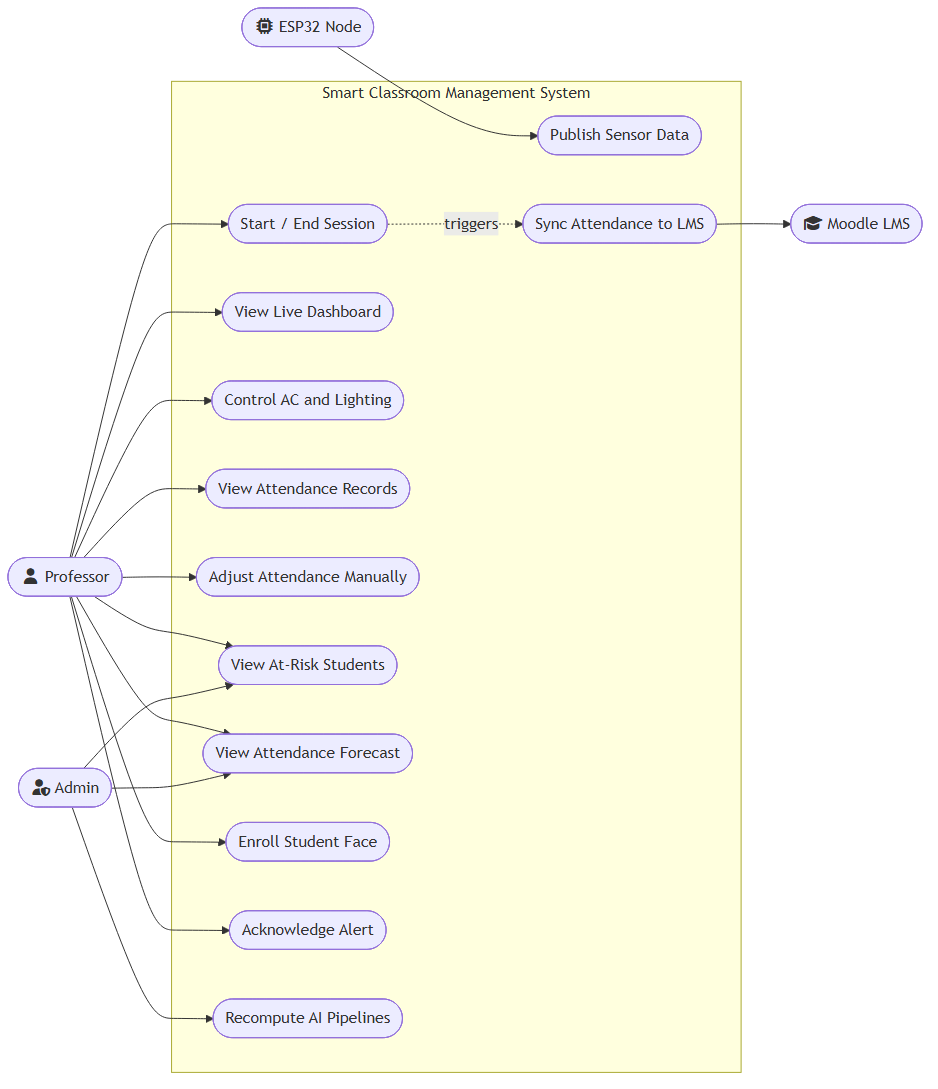
\includegraphics[width=\linewidth]{fig09_use_case}
  \caption{Use case diagram showing four actors and twelve use cases.}
  \label{fig:use_case}
\end{figure}

The critical use case sequence for a normal lecture is:
(1)~Professor starts session $\rightarrow$ (2)~Face recognition loop
activates $\rightarrow$ (3)~Attendance records update live on dashboard
$\rightarrow$ (4)~Professor ends session $\rightarrow$ (5)~Final absent
fill runs $\rightarrow$ (6)~Attendance syncs to Moodle.

\subsection{Constraints}
\label{subsec:constraints}

\textbf{Hardware constraints.}  The Raspberry Pi~4B (4~GB RAM) is the
sole compute node.  Face recognition is limited to 2~fps; phi3-mini
inference runs at 10--30~seconds per student on CPU.

\textbf{Budget constraints.}  Total hardware cost is approximately
\$150~USD, including the RPi~4B, ESP32, sensors, relay module, and
camera.  See Table~\ref{tab:hardware_bom} in
Section~\ref{subsec:hardware} for the detailed bill of materials.

\textbf{Timeline constraint.}  The project was delivered within one
academic semester (22 weeks, 22 phases).  Features deferred to future
work include multi-room support, HTTPS/WSS, and quantised GGUF model
inference.

%% ════════════════════════════════════════════════════════════════════════════
\section{System Architecture}
\label{sec:architecture}
%% ════════════════════════════════════════════════════════════════════════════

\subsection{Architecture Overview}
\label{subsec:arch_overview}

The system follows a \emph{hybrid modular monolith with event-driven
messaging} architecture.  The backend is a single FastAPI process; however,
it is internally structured around three decoupled event channels: an MQTT
ingestion pipeline, a WebSocket fan-out layer, and an on-demand AI
pipeline bus.  This avoids the operational overhead of microservices while
preserving the loose coupling that makes each subsystem independently
testable.

Figure~\ref{fig:arch_overview} shows the five-tier logical view: IoT
devices at the edge, a Mosquitto message broker, the FastAPI backend with
its service groups, the React frontend, and external integrations
(Moodle, Ollama).

\begin{figure}[H]
  \centering
  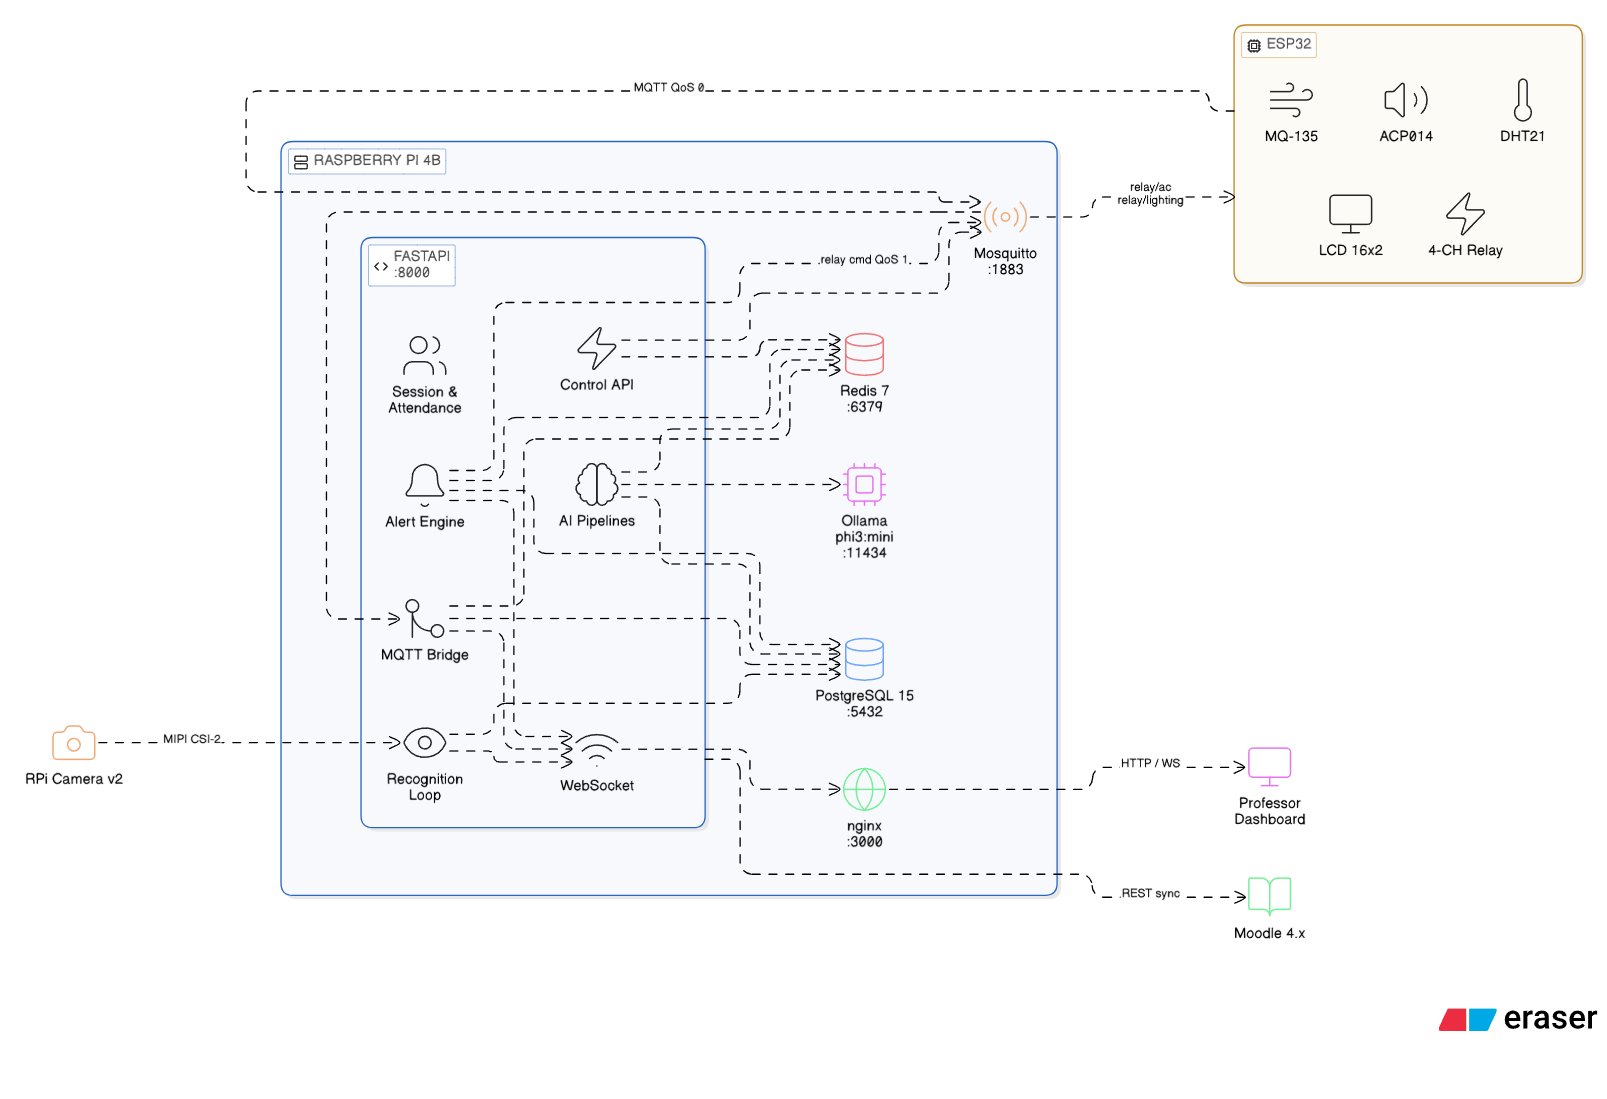
\includegraphics[width=\linewidth]{fig01_system_architecture}
  \caption{Full system layered architecture: IoT $\rightarrow$ Edge
    $\rightarrow$ Backend $\rightarrow$ Frontend $\rightarrow$ External.}
  \label{fig:arch_overview}
\end{figure}

Table~\ref{tab:tech_stack} summarises the technology choices for each
layer, and Table~\ref{tab:subsystems} lists each subsystem's primary
responsibility.

\begin{table}[H]
\centering
\caption{Technology Stack Summary}
\label{tab:tech_stack}
\begin{tabular}{@{}p{1.8cm}p{2.2cm}p{3.5cm}@{}}
\toprule
\textbf{Layer} & \textbf{Technology} & \textbf{Key Libraries} \\
\midrule
Firmware    & Arduino C++    & PubSubClient, DHT, LiquidCrystal\_I2C \\
Backend     & Python 3.11    & FastAPI, SQLAlchemy 2.0, aiomqtt, APScheduler, httpx \\
Database    & PostgreSQL 15  & Alembic (migrations) \\
Cache       & Redis 7        & redis-py async \\
AI          & Ollama phi3-mini & httpx AsyncClient \\
Face Rec.   & DeepFace       & OpenCV, FaceNet, numpy \\
Frontend    & React 18       & Vite, TailwindCSS, Recharts, axios \\
Infra       & Docker Compose & nginx, eclipse-mosquitto:2 \\
\bottomrule
\end{tabular}
\end{table}

\begin{table}[H]
\centering
\caption{Subsystem Responsibilities}
\label{tab:subsystems}
\begin{tabular}{@{}p{2.0cm}p{5.5cm}@{}}
\toprule
\textbf{Subsystem} & \textbf{Responsibility} \\
\midrule
IoT (ESP32)        & Sense environment; publish MQTT; actuate relays \\
Edge (RPi)         & Run all services locally; no cloud dependency \\
MQTT Broker        & Message bus between ESP32 and backend \\
Backend (FastAPI)  & Orchestration, REST + WebSocket APIs, business logic \\
Real-time Layer    & Fan-out of sensor/attendance/alert events to browsers \\
AI/Insights Layer  & At-risk detection, forecasting, SQL analytics \\
Frontend (React)   & Professor dashboard; demo mode when offline \\
Data Layer         & PostgreSQL (durable) + Redis (ephemeral live state) \\
External           & Moodle LMS sync; Ollama LLM inference \\
\bottomrule
\end{tabular}
\end{table}

%% ────────────────────────────────────────────────────────────────────────────
\subsection{IoT Layer — ESP32 Firmware}
\label{subsec:iot_layer}

\subsubsection{Sensor Acquisition}
The ESP32-WROOM-32 runs an Arduino sketch that reads four sensors on a
5-second cycle: the DHT21 temperature/humidity sensor (GPIO~4), the
MQ-135 air-quality ADC (GPIO~34, ADC1 channel~6), and the ACP014
digital sound sensor (GPIO~35).  GPIO~34 and~35 are input-only pins,
which avoids conflicts with the WiFi subsystem that disables ADC2.

\subsubsection{MQTT Publishing}
Each reading is serialised as a JSON payload
\texttt{\{value, unit, ts\}} and published to the corresponding MQTT
topic at QoS~0.  A heartbeat message (\texttt{status} topic, every
30~seconds) allows the backend to detect device offline events via a
TTL-based Redis presence key.

\subsubsection{Relay Actuation and Local Auto-Control}
The ESP32 subscribes to \texttt{classroom/room1/relay/ac} and
\texttt{classroom/room1/relay/lighting}.  On receipt, it drives the
corresponding GPIO output through a logic-level converter
(3.3\,V~$\leftrightarrow$\,5\,V) to the 4-channel opto-isolated relay
module.  An on-device auto-control flag (\texttt{acAutoMode}) implements
temperature thresholding independently of the backend---a deliberate
redundancy that maintains AC control if MQTT connectivity drops.

Figure~\ref{fig:esp32_wiring} shows the complete GPIO wiring.

\begin{figure}[H]
  \centering
  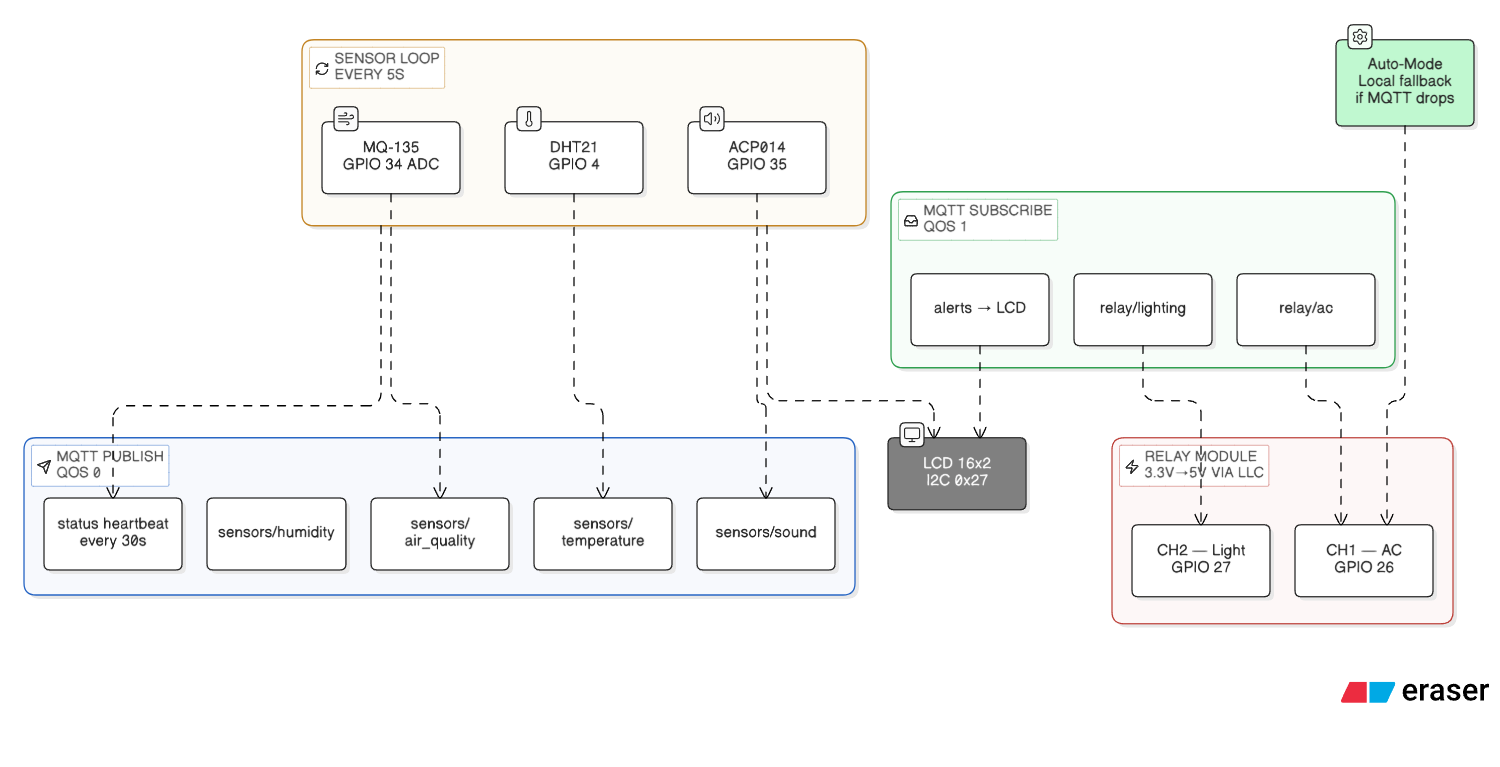
\includegraphics[width=\linewidth]{fig02_esp32_wiring}
  \caption{ESP32 IoT node: sensor inputs, logic-level converter, relay
    module, and LCD~16$\times$2 wiring.}
  \label{fig:esp32_wiring}
\end{figure}

%% ────────────────────────────────────────────────────────────────────────────
\subsection{Edge Layer — Raspberry Pi 4B}
\label{subsec:edge_layer}

The Raspberry Pi~4B (4~GB RAM) acts as the central edge hub, running
all Docker services on a single host.  In production, the RPi also
hosts the RPi Camera Module~v2, which feeds the face-recognition loop
at 2~fps via OpenCV \texttt{VideoCapture(0)}.

When \texttt{FACE\_RECOGNITION\_ENABLED=false} (Docker/dev mode), a
stub recognition loop fires synthetic attendance events using randomly
sampled enrolled students, exercising the full bidirectional
present$\leftrightarrow$absent evaluation logic without a physical
camera.

Figure~\ref{fig:rpi_topology} illustrates the runtime topology on the
Raspberry Pi~4B, including all Docker service ports and the WiFi link
to the ESP32 node.

\begin{figure}[H]
  \centering
  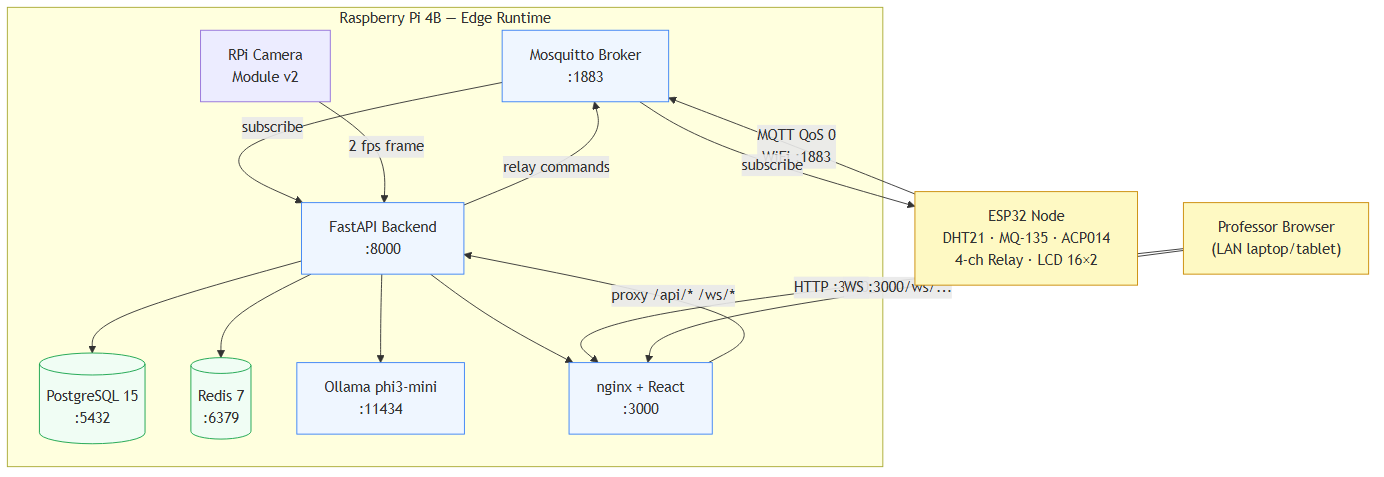
\includegraphics[width=\linewidth]{fig08_rpi_topology}
  \caption{RPi~4B production runtime topology: all services and their
    communication paths to the ESP32 classroom node and professor
    browser.}
  \label{fig:rpi_topology}
\end{figure}

%% ────────────────────────────────────────────────────────────────────────────
\subsection{Communication Layer — MQTT}
\label{subsec:mqtt_layer}

\subsubsection{Topic Architecture}
The Mosquitto~2 broker hosts a single hierarchical topic tree under the
prefix \texttt{classroom/\{room\_id\}/}.  Table~\ref{tab:mqtt_schema}
defines all topics, directions, and payload schemas.

\begin{table}[H]
\centering
\caption{MQTT Topic Schema}
\label{tab:mqtt_schema}
\begin{tabular}{@{}p{2.8cm}p{1.1cm}p{3.6cm}@{}}
\toprule
\textbf{Topic suffix} & \textbf{Dir.} & \textbf{Payload / Period} \\
\midrule
\texttt{sensors/temperature} & ESP$\rightarrow$RPi & \texttt{\{value,unit,ts\}} · 5~s \\
\texttt{sensors/humidity}    & ESP$\rightarrow$RPi & \texttt{\{value,unit,ts\}} · 5~s \\
\texttt{sensors/air\_quality}& ESP$\rightarrow$RPi & \texttt{\{value,unit,ts\}} · 5~s \\
\texttt{sensors/sound}       & ESP$\rightarrow$RPi & \texttt{\{value:0|1,ts\}} · 5~s \\
\texttt{status}              & ESP$\rightarrow$RPi & \texttt{\{online:true,ts\}} · 30~s \\
\texttt{relay/ac}            & RPi$\rightarrow$ESP & \texttt{\{action:on|off|auto\}} \\
\texttt{relay/lighting}      & RPi$\rightarrow$ESP & \texttt{\{action:on|off|auto\}} \\
\texttt{alerts}              & RPi$\rightarrow$ESP & \texttt{\{type,value\}} $\rightarrow$ LCD \\
\bottomrule
\end{tabular}
\end{table}

\subsubsection{Subscription Strategy}
The backend subscribes using the wildcard pattern
\texttt{classroom/+/sensors/\#} to receive sensor messages from any
room ID and any sensor sub-topic in a single subscription.  A separate
subscription on \texttt{classroom/+/status} handles heartbeat messages.
ESP32 nodes subscribe to exact topics for relay commands.

Figure~\ref{fig:mqtt_topics} shows the complete topic tree.

\begin{figure}[H]
  \centering
  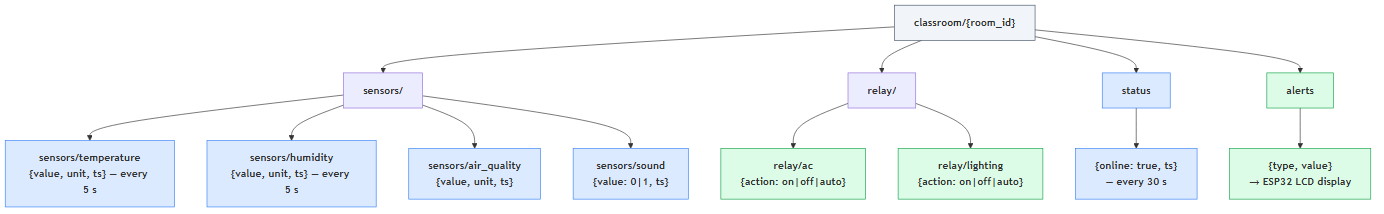
\includegraphics[width=\linewidth]{fig03_mqtt_topic_tree}
  \caption{MQTT topic tree under \texttt{classroom/\{room\_id\}/}.
    Blue nodes are ESP32-published; green nodes are backend-published.}
  \label{fig:mqtt_topics}
\end{figure}

%% ────────────────────────────────────────────────────────────────────────────
\subsection{Backend — FastAPI Application}
\label{subsec:backend}

The backend is organised into seven logical service groups.
Figure~\ref{fig:backend_modules} shows their connections.

\begin{figure}[H]
  \centering
  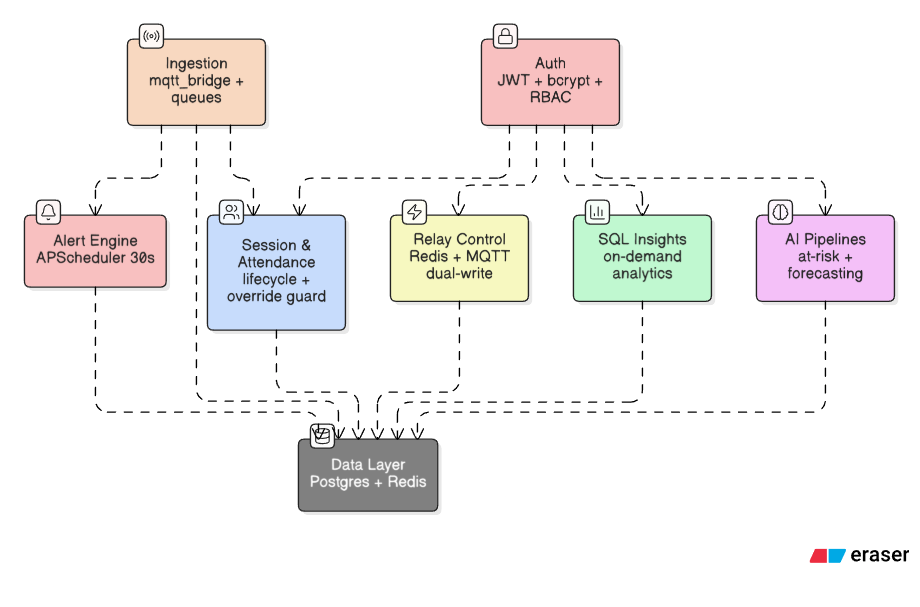
\includegraphics[width=\linewidth]{fig04_backend_modules}
  \caption{Backend internal module groups and their data-flow
    connections.}
  \label{fig:backend_modules}
\end{figure}

\textbf{Group~1 — Ingestion \& Real-time} (\texttt{mqtt\_bridge.py}).
A persistent \texttt{aiomqtt.Client} subscriber loop connects to
Mosquitto with exponential backoff.  On each sensor message: (i)~Redis
SET with 5-minute TTL, (ii)~fire-and-forget PostgreSQL write,
(iii)~non-blocking put to \texttt{sensor\_event\_queue}.  Three
\texttt{asyncio.Queue} instances decouple producers from WebSocket
consumers.

\textbf{Group~2 — Session \& Attendance} (\texttt{api/sessions.py},
\texttt{recognition\_loop.py}).  Session lifecycle: \texttt{POST
/api/sessions/start} activates the recognition loop; \texttt{POST
/api/sessions/\{id\}/end} stops it, runs the final evaluation cycle,
and triggers Moodle sync.  Manual adjustments via
\texttt{PATCH /api/attendance/\{id\}} set \texttt{adjusted\_by} to
prevent overwrite by the recognition loop.

\textbf{Group~3 — Control} (\texttt{api/control.py}).  Relay commands
simultaneously write Redis (instant dashboard state) and publish MQTT
(device actuation).  Redis is the authoritative relay state; PostgreSQL
is not used for relay records.

\textbf{Group~4 — Alert Engine} (\texttt{services/alert\_engine.py}).
An \texttt{AsyncIOScheduler} job runs every 30~seconds, reads the Redis
sensor cache, evaluates thresholds (Table~\ref{tab:auto_control}), and
upserts \texttt{alerts} rows.  Deduplication prevents duplicate alerts
for the same unacknowledged condition.

\textbf{Group~5 — Insights \& Analytics.}  Pure SQL analytics: weekly
trend, day/hour heatmap, comfort score, AC effectiveness, temperature
versus attendance scatter, air-quality versus sound correlation.
Role-filtered: professors see only their courses.

\textbf{Group~6 — AI Pipelines} (Section~\ref{sec:ai}).

\textbf{Group~7 — Auth} (\texttt{api/auth.py}).  JWT (HS256), bcrypt
passwords, role-based access control; \texttt{REQUIRE\_AUTH=false} in
development.

\begin{table}[H]
\centering
\caption{Auto-Control Rules}
\label{tab:auto_control}
\begin{tabular}{@{}p{1.6cm}p{2.4cm}p{3.5cm}@{}}
\toprule
\textbf{Sensor} & \textbf{Condition} & \textbf{Action} \\
\midrule
Temperature & $> 28$\,°C + AC in auto & Turn AC ON \\
Temperature & $< 22$\,°C + AC in auto & Turn AC OFF \\
Air quality & $> 500$~ppm            & Alert (no relay) \\
Sound       & Silent $> 30$~min (active session) & Attendance anomaly alert \\
Device      & Heartbeat TTL expired  & Device-offline alert \\
\bottomrule
\end{tabular}
\end{table}

\begin{table}[H]
\centering
\caption{APScheduler Job Inventory}
\label{tab:scheduler_jobs}
\begin{tabular}{@{}p{2.8cm}p{1.1cm}p{3.6cm}@{}}
\toprule
\textbf{Job} & \textbf{Interval} & \textbf{Purpose} \\
\midrule
\texttt{check\_thresholds} & 30~s & Sensor threshold evaluation, relay auto-control, alert creation \\
\texttt{retry\_moodle\_sync} & 10~min & Re-send up to 10 queued session IDs to Moodle \\
\texttt{mock\_sensor\_publish} & 5~s & (\texttt{MOCK\_MODE}) Synthetic MQTT sensor messages \\
\texttt{mock\_heartbeat} & 30~s & (\texttt{MOCK\_MODE}) Synthetic status heartbeat \\
\bottomrule
\end{tabular}
\end{table}

Table~\ref{tab:api_endpoints} lists the primary REST endpoints.

\begin{table}[H]
\centering
\caption{Primary REST API Endpoints}
\label{tab:api_endpoints}
\begin{tabular}{@{}p{0.8cm}p{3.8cm}p{2.9cm}@{}}
\toprule
\textbf{Method} & \textbf{Path} & \textbf{Description} \\
\midrule
GET  & \texttt{/api/sensors/latest}            & Latest sensor values (Redis) \\
GET  & \texttt{/api/sensors/history}           & Time-range history (PG) \\
POST & \texttt{/api/sessions/start}            & Create + start session \\
POST & \texttt{/api/sessions/\{id\}/end}       & End session, sync Moodle \\
POST & \texttt{/api/control/ac}                & Set AC relay state \\
POST & \texttt{/api/control/lighting}          & Set lighting relay state \\
GET  & \texttt{/api/sessions/\{id\}/attendance}& Attendance roster \\
PATCH& \texttt{/api/attendance/\{id\}}         & Manual adjustment \\
POST & \texttt{/api/students/\{id\}/enroll-face}& Face enrollment \\
GET  & \texttt{/api/at-risk}                   & At-risk list + trigger pipeline \\
GET  & \texttt{/api/forecasting}               & Forecast list + trigger pipeline \\
WS   & \texttt{/ws/classroom/\{room\_id\}}     & Live event stream \\
\bottomrule
\end{tabular}
\end{table}

%% ────────────────────────────────────────────────────────────────────────────
\subsection{Real-Time Layer — WebSocket}
\label{subsec:websocket}

Figure~\ref{fig:ws_fanout} shows the asyncio fan-out mechanism.  Three
background drain tasks loop indefinitely, pulling events from their
respective queues and calling \texttt{connection\_manager.broadcast(room\_id,
event)}.  The \texttt{ConnectionManager} maintains a
\texttt{dict[room\_id $\rightarrow$ set[WebSocket]]} for room-scoped
delivery.

\begin{figure}[H]
  \centering
  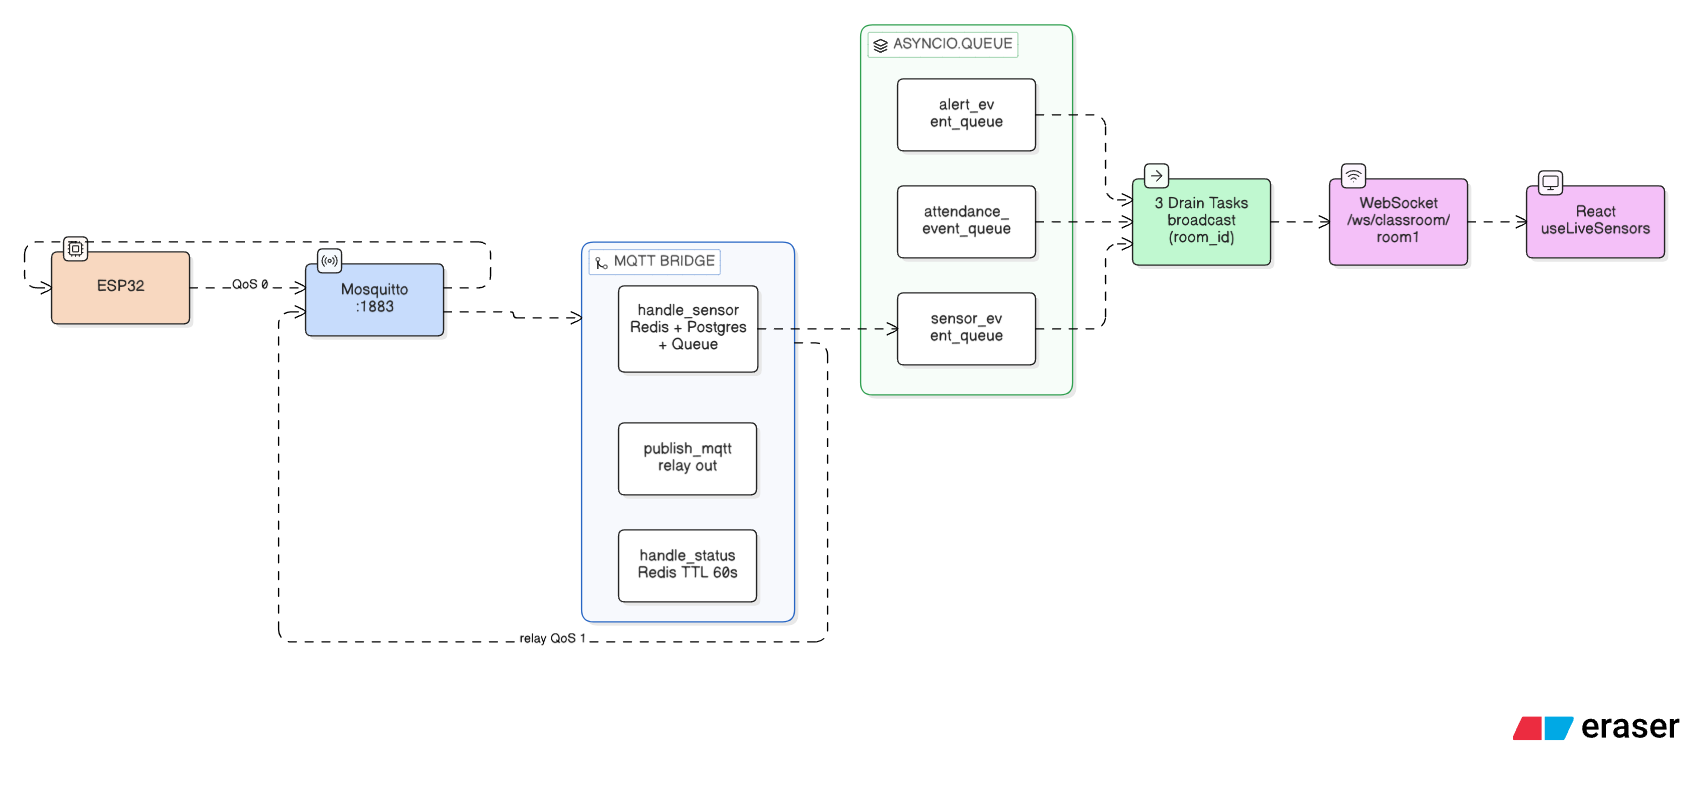
\includegraphics[width=\linewidth]{fig05_websocket_fanout}
  \caption{Event fan-out: three asyncio queues drain independently into
    the WebSocket broadcast layer.}
  \label{fig:ws_fanout}
\end{figure}

On connect, the server immediately sends a \texttt{snapshot} message
containing current Redis sensor values, relay states, and device-online
status, ensuring the dashboard is never blank on page load.  A
30-second server-side keepalive (ping/pong) detects stale connections.
The frontend reconnects with exponential backoff (3~s initial, 30~s
cap).  Table~\ref{tab:ws_messages} defines all WebSocket message types.

\begin{table}[H]
\centering
\caption{WebSocket Message Types (Server $\rightarrow$ Client)}
\label{tab:ws_messages}
\begin{tabular}{@{}p{1.5cm}p{2.4cm}p{3.6cm}@{}}
\toprule
\textbf{Type} & \textbf{Trigger} & \textbf{Payload fields} \\
\midrule
\texttt{snapshot}   & On connect       & sensors, relay, device\_online \\
\texttt{sensor}     & MQTT ingestion   & room\_id, sensor\_type, value, unit \\
\texttt{attendance} & Recognition match & session\_id, student\_id, name, confidence, status \\
\texttt{alert}      & Threshold breach & alert\_type, room\_id, message, value \\
\texttt{ping}       & 30~s keepalive   & — \\
\bottomrule
\end{tabular}
\end{table}

%% ────────────────────────────────────────────────────────────────────────────
\subsection{Data Layer}
\label{subsec:data_layer}

\subsubsection{PostgreSQL Schema}
The database contains nine tables.
Figure~\ref{fig:er_diagram} shows the entity-relationship diagram.

\begin{figure}[H]
  \centering
  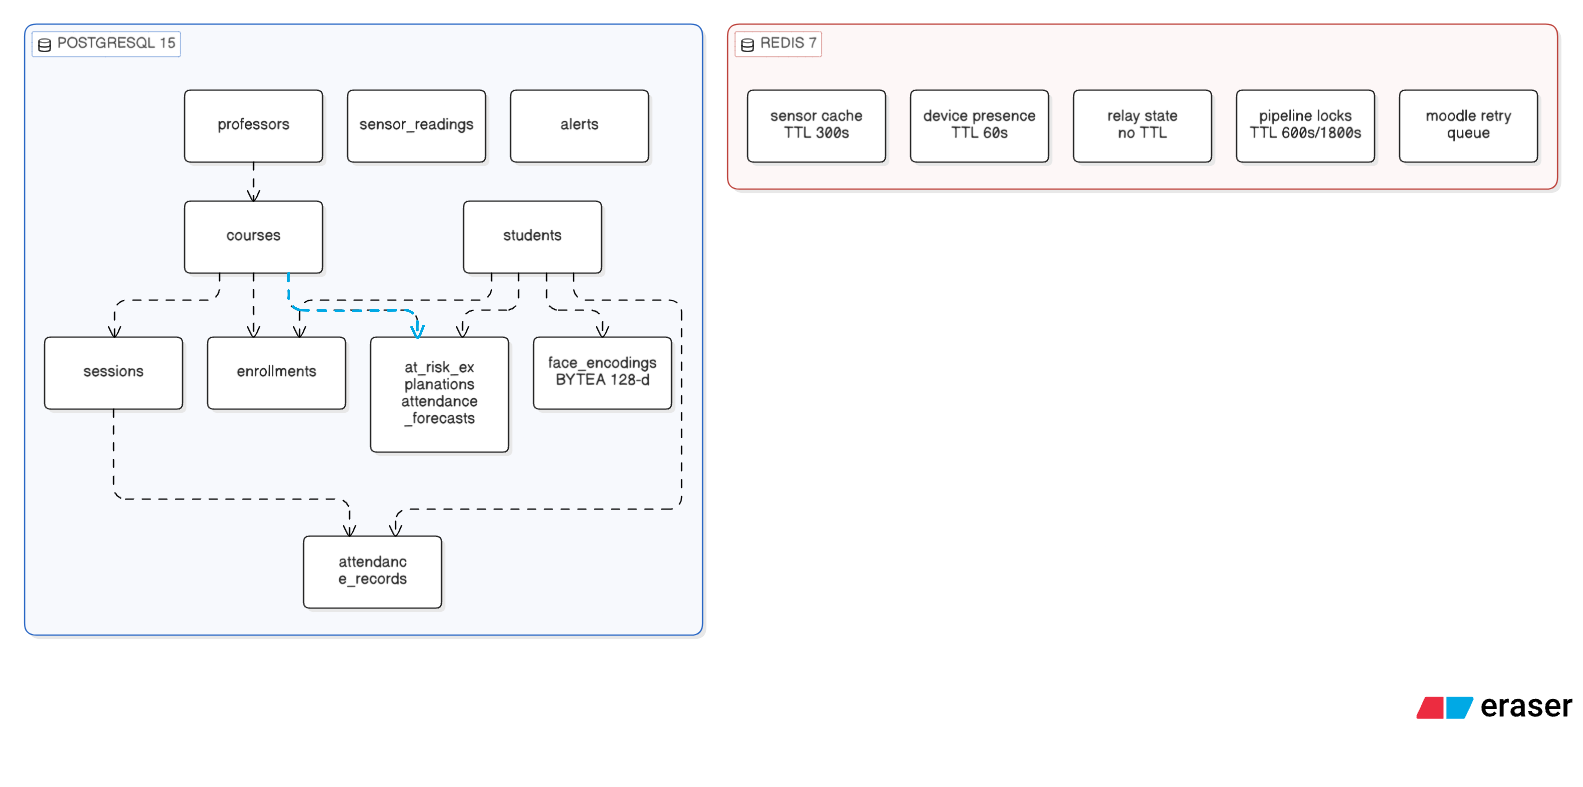
\includegraphics[width=\linewidth]{fig06_er_diagram}
  \caption{Entity-relationship diagram for all nine database tables.}
  \label{fig:er_diagram}
\end{figure}

Table~\ref{tab:db_schema} summarises each table's purpose and key
design decisions.

\begin{table}[H]
\centering
\caption{Database Schema Summary}
\label{tab:db_schema}
\begin{tabular}{@{}p{2.5cm}p{5.0cm}@{}}
\toprule
\textbf{Table} & \textbf{Key Design Points} \\
\midrule
\texttt{professors}        & UUID PK, bcrypt password, role ENUM (professor|admin) \\
\texttt{students}          & UUID PK, UNIQUE institutional student\_id \\
\texttt{courses}           & UUID PK, UNIQUE code, nullable professor FK \\
\texttt{sessions}          & display\_status computed (not stored) to reflect live state \\
\texttt{attendance\_records} & adjusted\_by guard: recognition loop never overwrites manual changes \\
\texttt{face\_encodings}   & 128-d float32 BYTEA; no raw images stored \\
\texttt{sensor\_readings}  & Time-series; queried for history and AI pipeline sensor averages \\
\texttt{at\_risk\_explanations} & UNIQUE student\_id; per\_course\_data as JSONB \\
\texttt{attendance\_forecasts} & UNIQUE course\_id; VARCHAR(30) for classification, not PG ENUM \\
\bottomrule
\end{tabular}
\end{table}

Key schema decisions: \texttt{display\_status} is computed at query time
because session liveness changes over time without a write.
\texttt{per\_course\_data} is JSONB because it is always read/written as
a unit with the parent row.  \texttt{trend\_classification} uses
\texttt{VARCHAR(30)} instead of a PostgreSQL ENUM to avoid
non-transactional \texttt{ALTER TYPE ADD VALUE} DDL on schema evolution.

\subsubsection{Redis Key Patterns}
Table~\ref{tab:redis_keys} defines all Redis key patterns, their
semantics, and TTL behaviour.

\begin{table}[H]
\centering
\caption{Redis Key Patterns}
\label{tab:redis_keys}
\begin{tabular}{@{}p{3.0cm}p{1.5cm}p{3.0cm}@{}}
\toprule
\textbf{Key pattern} & \textbf{TTL} & \textbf{Semantics} \\
\midrule
\texttt{classroom:\{r\}:sensors:\{t\}} & 300~s & Latest sensor value for type \texttt{t} \\
\texttt{classroom:\{r\}:online}        & 60~s  & Device presence (heartbeat-renewed) \\
\texttt{classroom:\{r\}:relay:\{d\}}   & None  & Relay state; persists across restarts \\
\texttt{at\_risk:pipeline:lock}        & 600~s & Prevents concurrent pipeline runs \\
\texttt{forecast:pipeline:lock}        & 1800~s & Prevents concurrent forecast runs \\
Moodle retry list                      & None  & Session IDs awaiting Moodle sync \\
\bottomrule
\end{tabular}
\end{table}

%% ────────────────────────────────────────────────────────────────────────────
\subsection{Frontend — React Dashboard}
\label{subsec:frontend}

The frontend is a single-page application (React~18, Vite, React
Router~v6).  Two context providers supply global state:
\texttt{AuthContext} (JWT token, professor profile) and
\texttt{SensorContext} (wrapping the \texttt{useLiveSensors} hook that
manages the WebSocket connection and demo-mode fallback).

The design system separates tokens from component classes:
\texttt{tokens.css} defines all CSS custom properties (colours,
spacing, radius, typography); \texttt{index.css} uses those variables
in component class rules.  TailwindCSS~v3 utility classes coexist but
cannot resolve CSS custom properties at build time, making the token
file split necessary.

Figures~\ref{fig:dashboard}--\ref{fig:control} show the three primary
professor-facing views.

\begin{figure}[H]
  \centering
  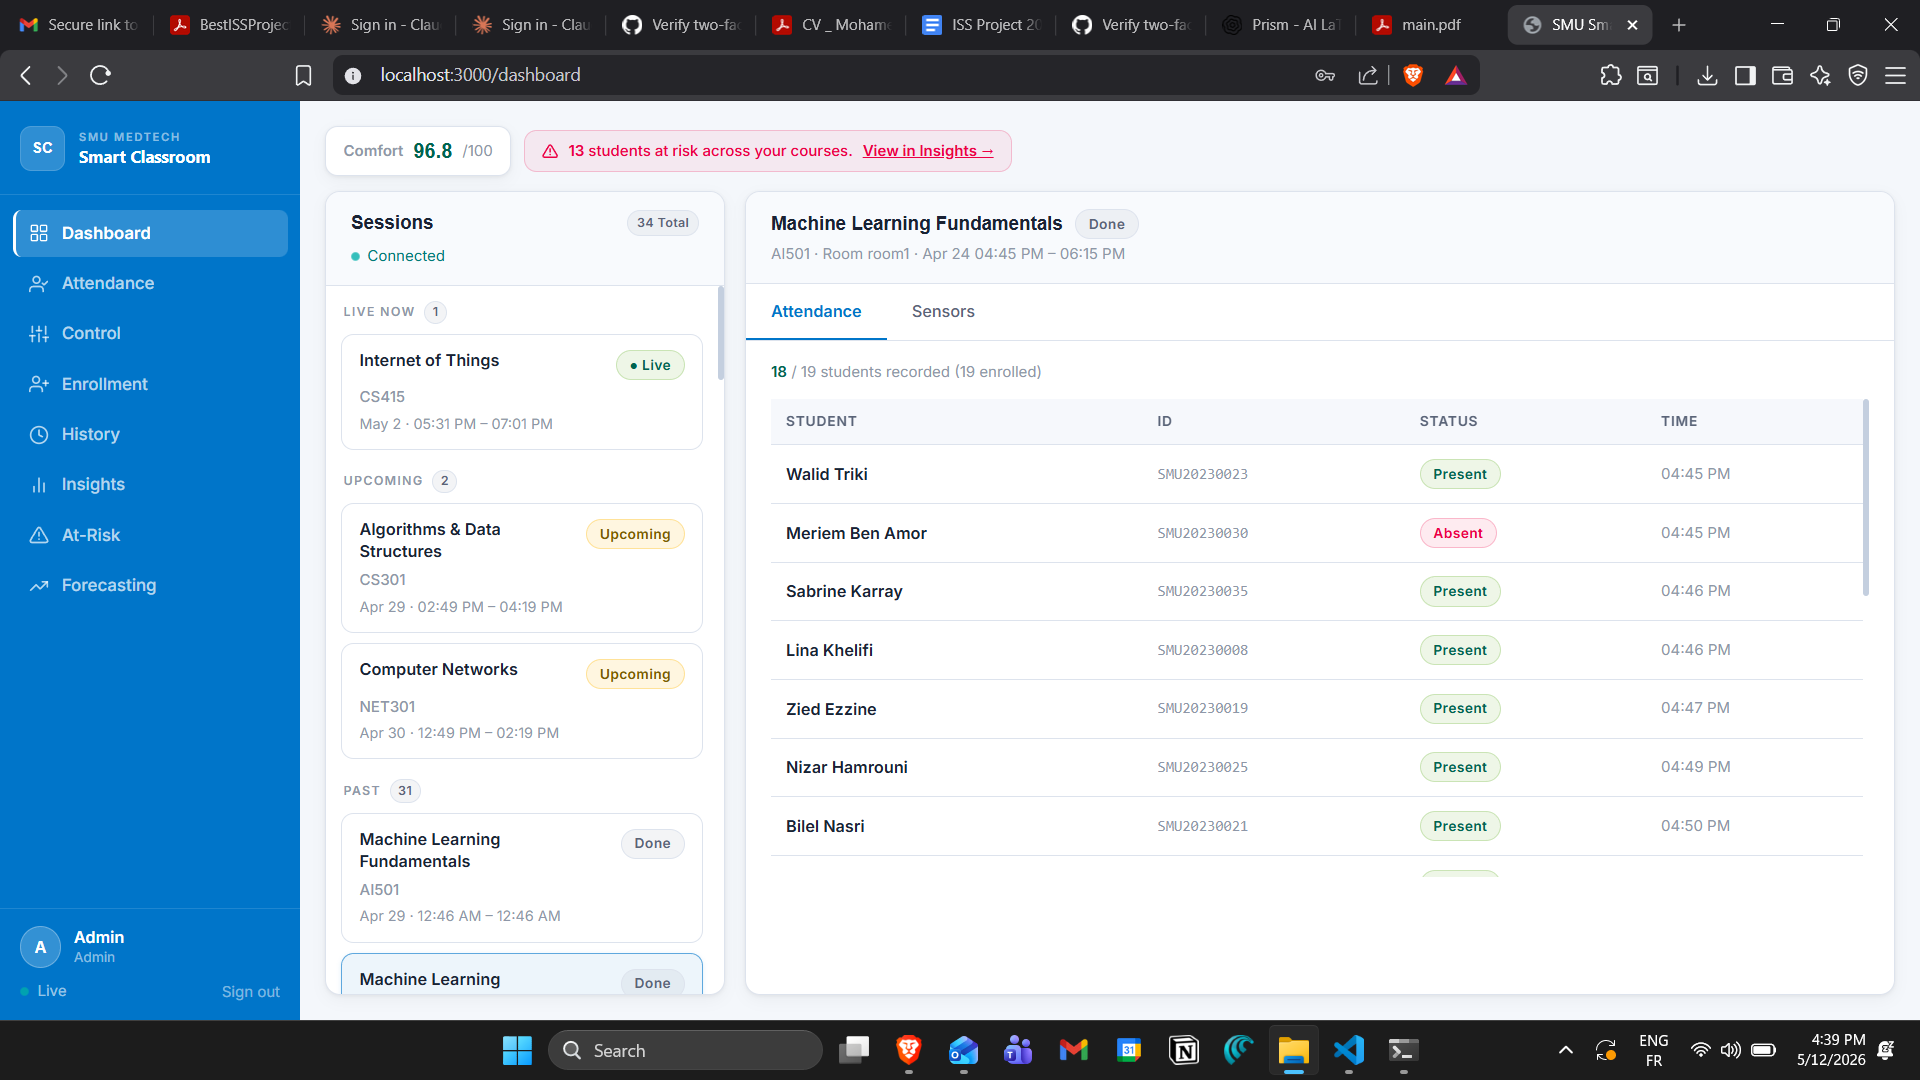
\includegraphics[width=\linewidth]{screenshot_dashboard}
  \caption{Dashboard page: live sensor sparklines, session control, and
    relay status cards.}
  \label{fig:dashboard}
\end{figure}

\begin{figure}[H]
  \centering
  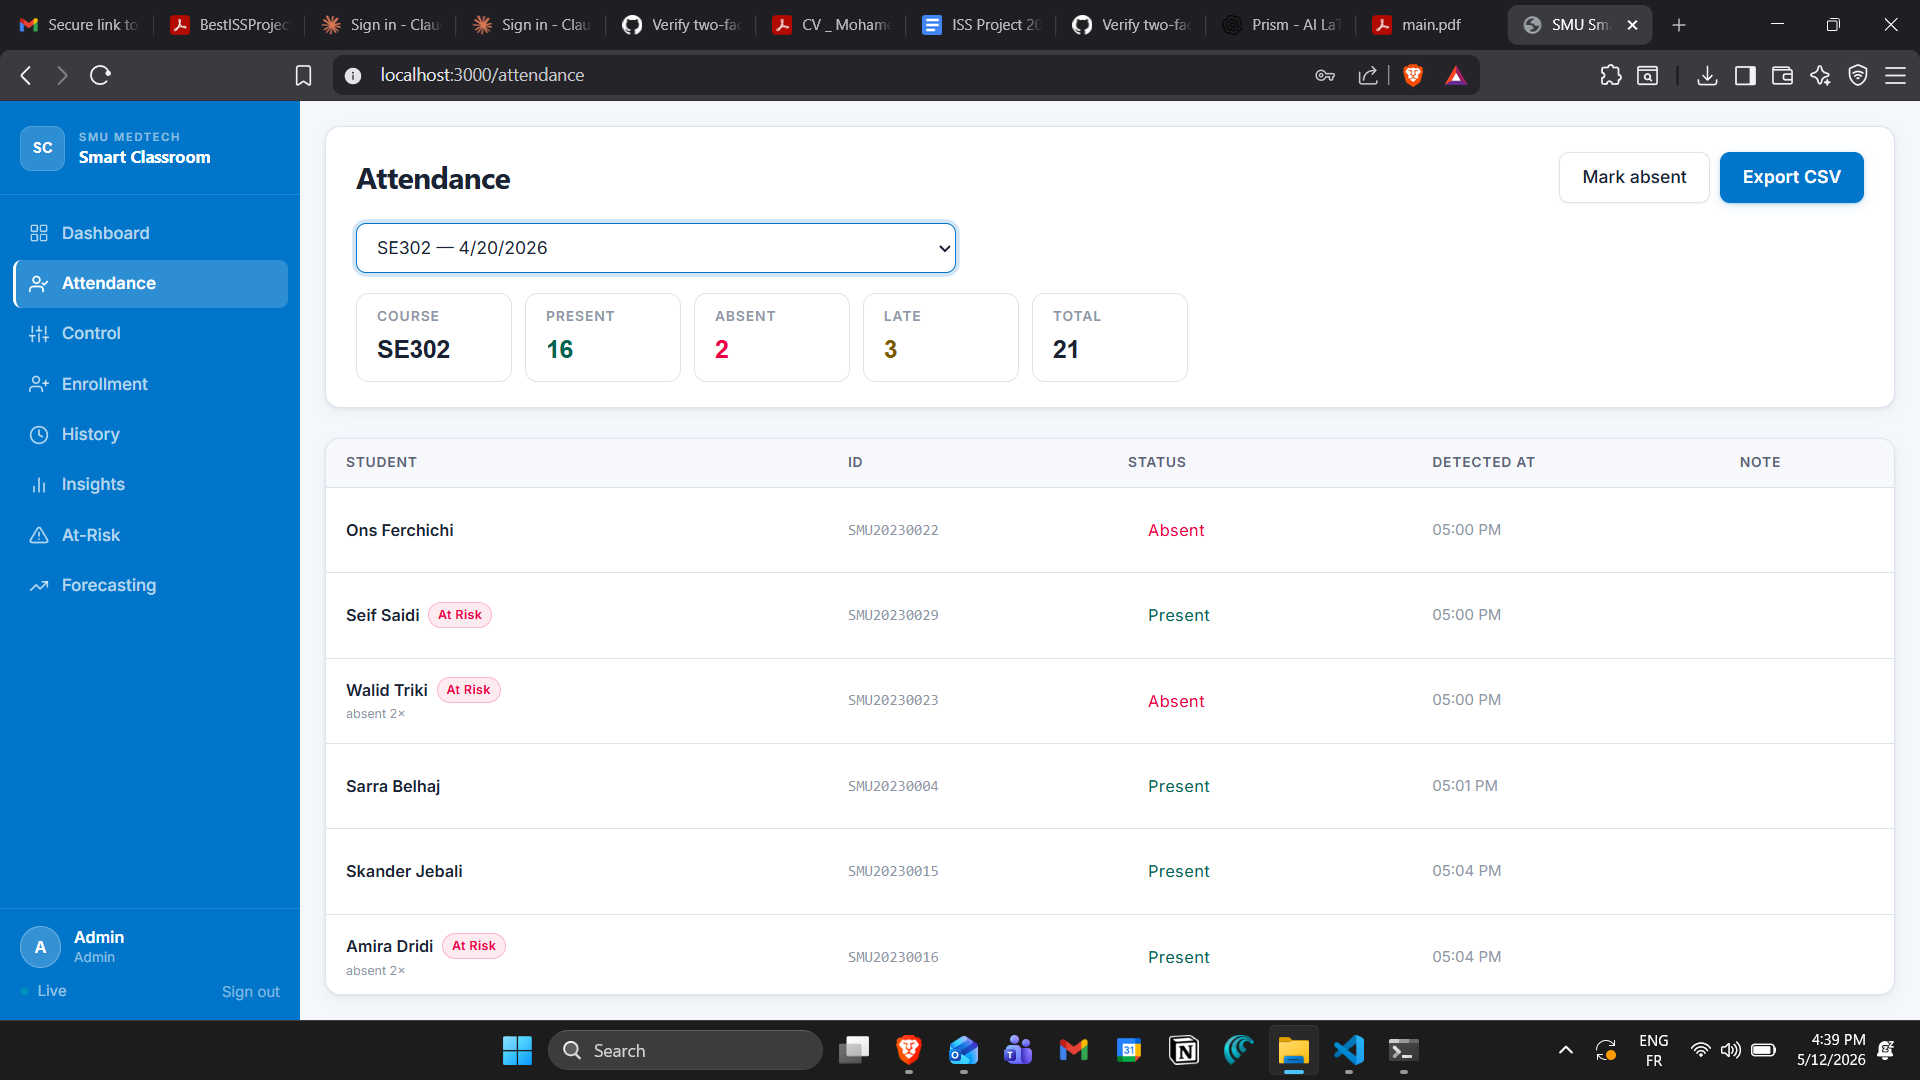
\includegraphics[width=\linewidth]{screenshot_attendance}
  \caption{Attendance page: per-student status table with manual
    adjustment capability.}
  \label{fig:attendance}
\end{figure}

\begin{figure}[H]
  \centering
  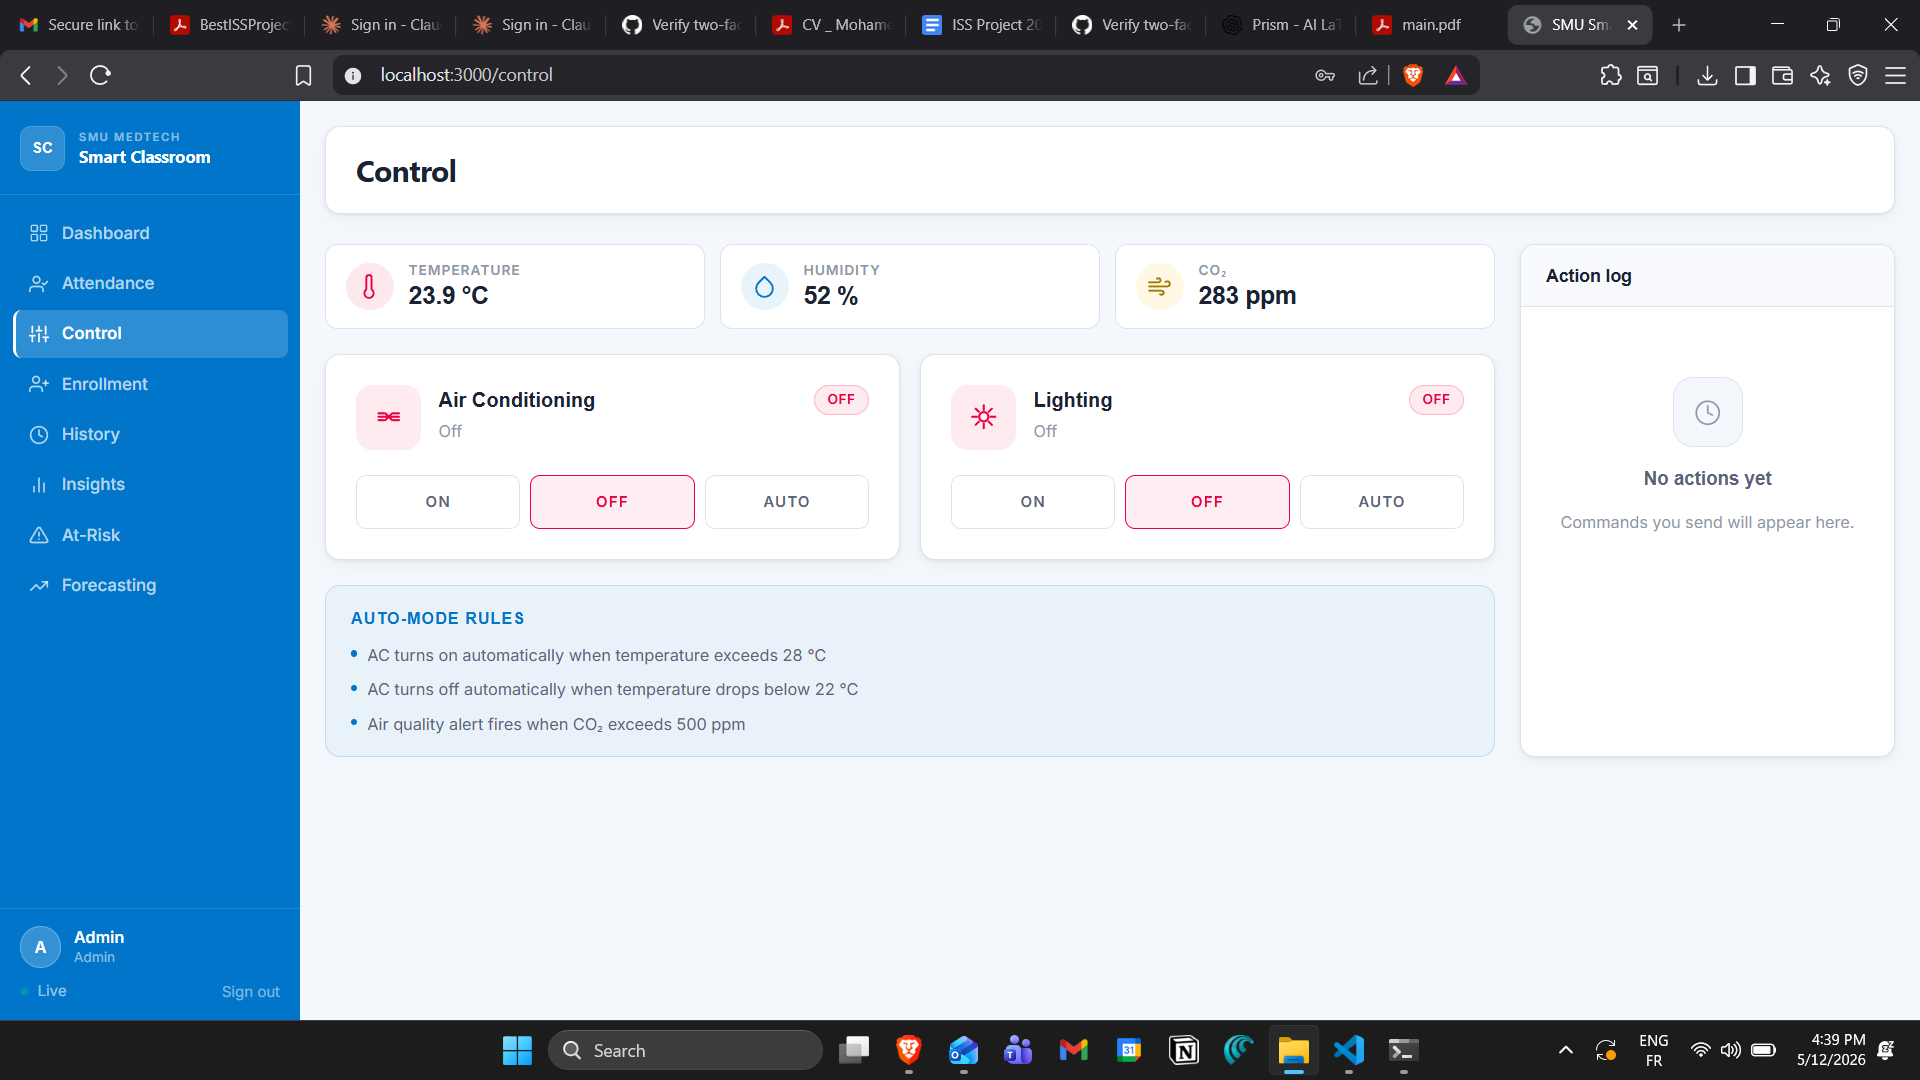
\includegraphics[width=\linewidth]{screenshot_control}
  \caption{Control page: relay toggle controls with live sensor summary
    cards.}
  \label{fig:control}
\end{figure}

%% ────────────────────────────────────────────────────────────────────────────
\subsection{External Integrations}
\label{subsec:external}

\textbf{Moodle 4.x.}  The optional Moodle integration calls the Moodle
REST API (token-authenticated) on session end to write attendance
records.  Failures are enqueued in Redis; the alert engine retries up
to 10 items every 10~minutes.  Moodle runs as an optional Docker Compose
profile to avoid adding 600~MB of container weight to the default
development environment.

\textbf{Ollama / phi3-mini.}  The Ollama service exposes a REST API at
\texttt{http://ollama:11434}.  On backend startup, an async background
task checks for the phi3:mini model via \texttt{GET /api/tags} and pulls
it (\texttt{POST /api/pull}) if absent---a non-blocking operation that
takes approximately 2~GB of download on first run.  Both AI pipelines
share a single \texttt{httpx.AsyncClient} to reuse TCP connections and
avoid per-call TCP handshake overhead.

%% ────────────────────────────────────────────────────────────────────────────
\subsection{Deployment Architecture}
\label{subsec:deployment}

Figure~\ref{fig:docker_compose} shows the Docker Compose service
dependency graph.  PostgreSQL and Redis must pass health checks before
the backend starts.  The frontend starts after the backend is running,
so that the nginx proxy target is always reachable.

\begin{figure}[H]
  \centering
  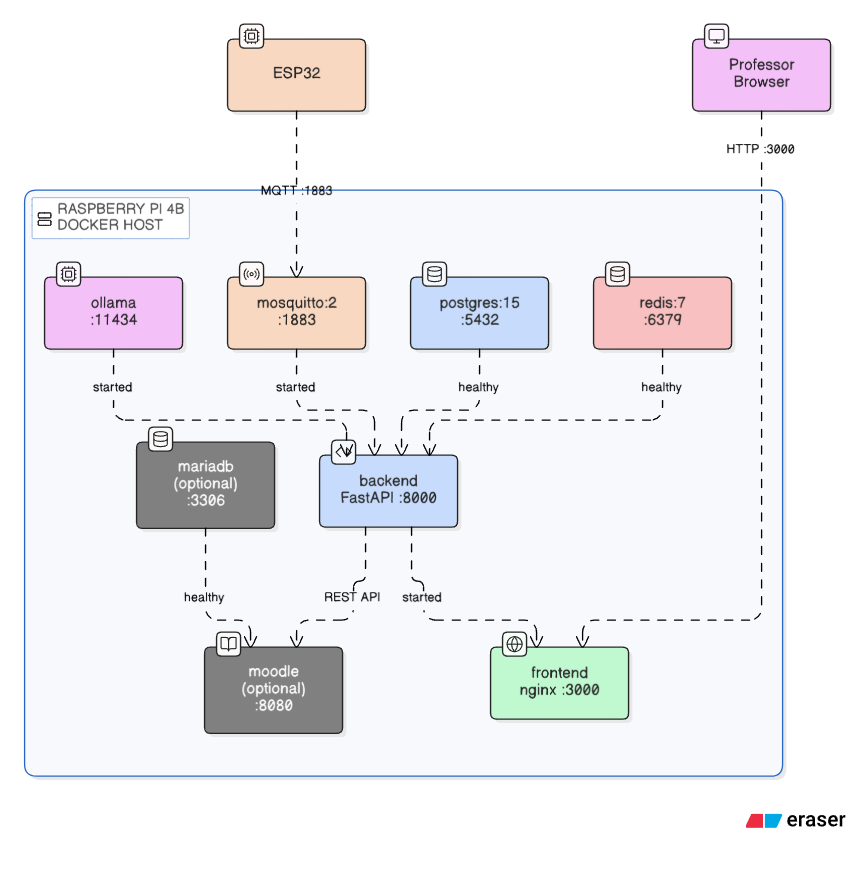
\includegraphics[width=\linewidth]{fig07_docker_compose}
  \caption{Docker Compose service graph showing dependency order and
    container image sources.}
  \label{fig:docker_compose}
\end{figure}

Alembic migrations run automatically in the FastAPI lifespan context
(\texttt{upgrade head}) before any API routes are registered, ensuring
schema currency on every container restart without a manual migration
step.

%% ────────────────────────────────────────────────────────────────────────────
\subsection{Key Architectural Decisions}
\label{subsec:arch_decisions}

Table~\ref{tab:arch_decisions} captures the most significant
non-obvious architectural choices and their rationale.

\begin{table}[H]
\centering
\caption{Key Architectural Decisions}
\label{tab:arch_decisions}
\begin{tabular}{@{}p{2.5cm}p{5.0cm}@{}}
\toprule
\textbf{Decision} & \textbf{Rationale} \\
\midrule
FastAPI over Flask          & Native async for WebSocket + MQTT concurrent I/O \\
All services on RPi         & Avoids latency, cost, and internet dependency \\
asyncio-mqtt $\rightarrow$ aiomqtt & paho-mqtt~v2 broke the asyncio-mqtt API \\
DeepFace stub in Docker     & TensorFlow adds $\sim$600~MB; causes OOM on dev laptops \\
Redis for sensor state      & Sub-millisecond read on page load; no PostgreSQL hit \\
\texttt{display\_status} computed & Liveness is time-relative; storing it would require continuous writes \\
\texttt{tokens.css} split   & TailwindCSS~v3 cannot resolve CSS vars at build time \\
Glassmorphism removed       & GPU-expensive; caused rendering artifacts in Chrome \\
Inline SVG icons            & No icon-library dependency; only 10--12 icons needed \\
\texttt{per\_course\_data} JSONB & Always read/written as a unit; avoids join \\
Redis TTL not deleted on completion & Prevents re-run on every page refresh (natural cooldown) \\
1~LLM call/student          & N+1 calls: 14--16~min; batched: 2--3~min \\
Deterministic classification & LLM labels are unreliable for structured values; delta math is deterministic \\
\texttt{VARCHAR(30)} not PG ENUM & \texttt{ALTER TYPE ADD VALUE} is non-transactional in PostgreSQL \\
Marker rows ($<3$ sessions)  & Without a row, the frontend poll condition never resolves \\
No Redis cooldown in webcam endpoint & \texttt{last\_posted\_status} in the laptop script is the dedup layer; backend cooldown silently dropped transitions \\
\bottomrule
\end{tabular}
\end{table}

%% ════════════════════════════════════════════════════════════════════════════
\section{Implementation}
\label{sec:implementation}
%% ════════════════════════════════════════════════════════════════════════════

\subsection{Development Methodology and Task Management}
\label{subsec:methodology}

The project followed an Agile-inspired iterative delivery model,
organised into 22 numbered phases spanning hardware assembly, firmware,
backend services, frontend, Docker deployment, and AI analytics.  Each
phase had a clear definition of done and was tracked on a shared Notion
board.  Figure~\ref{fig:notion} shows the task board at the time of
final submission.

\begin{figure}[H]
  \centering
  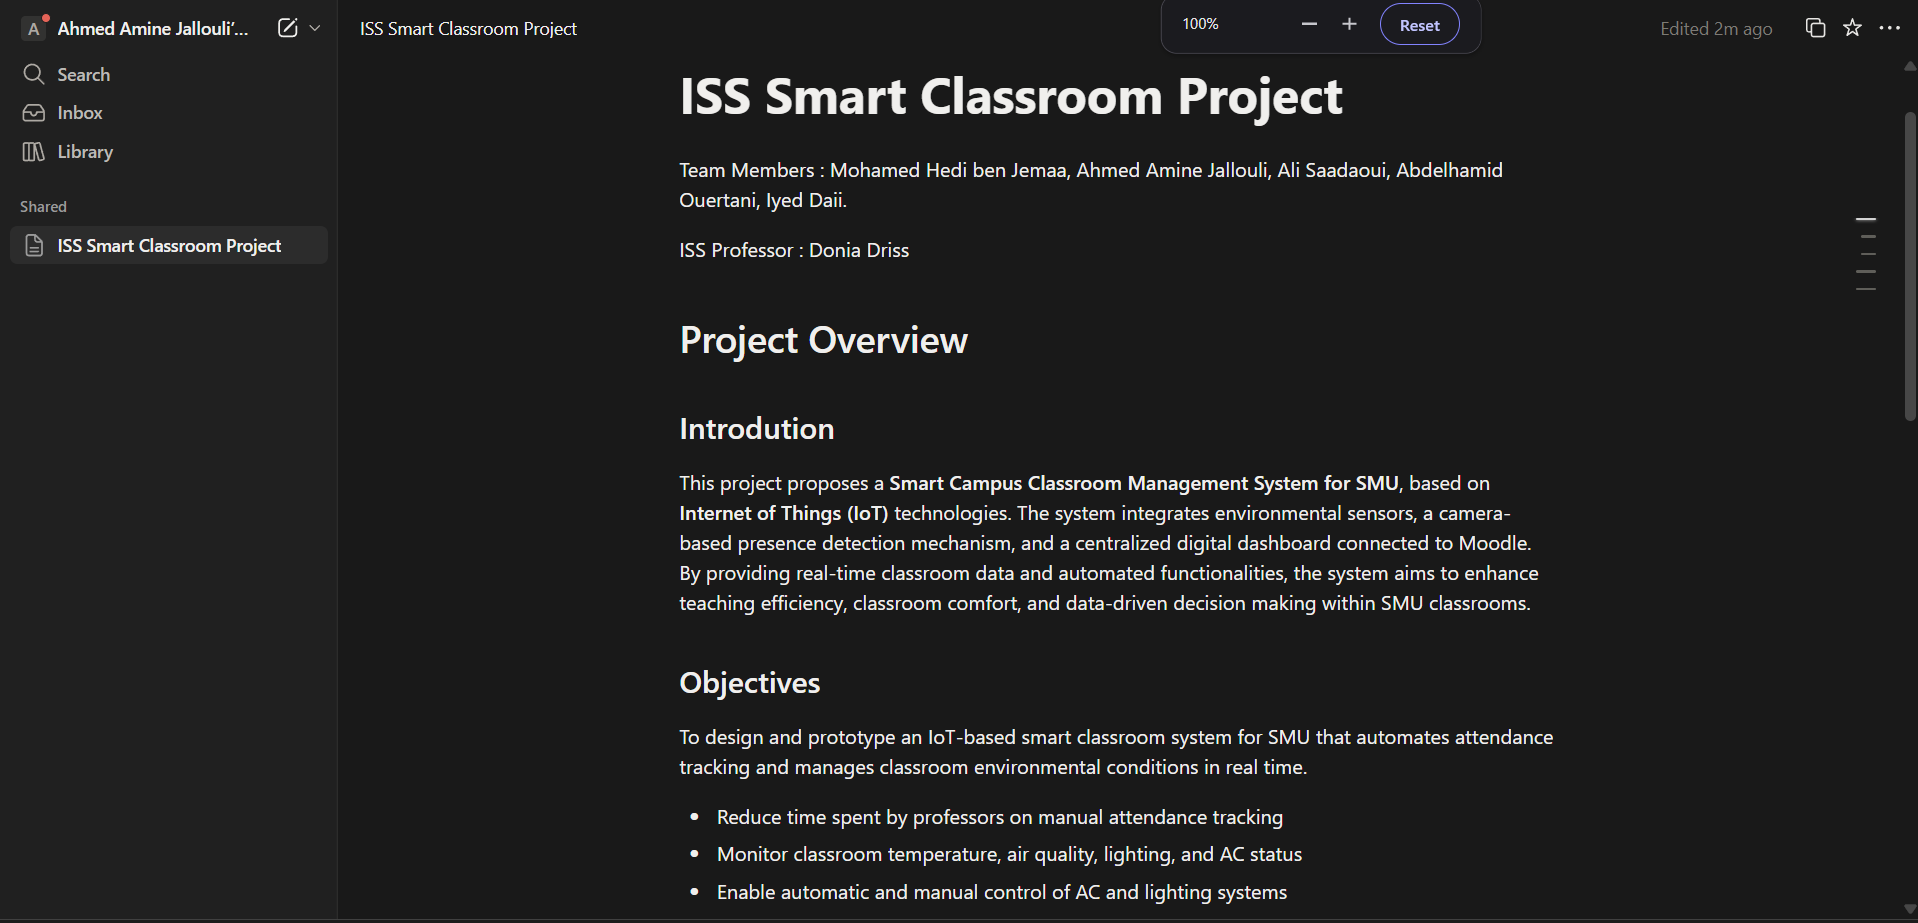
\includegraphics[width=\linewidth]{screenshot_notion}
  \caption{Notion project board: phase breakdown, assignee tracking,
    and completion status.}
  \label{fig:notion}
\end{figure}

Table~\ref{tab:phases} shows the 22 delivery phases and their
completion status.

\begin{table}[H]
\centering
\caption{Phase Completion Status}
\label{tab:phases}
\begin{tabular}{@{}p{0.6cm}p{6.6cm}p{0.5cm}@{}}
\toprule
\textbf{Ph.} & \textbf{Description} & \textbf{Done} \\
\midrule
0  & Project scaffolding, Docker Compose, env setup         & \checkmark \\
1  & ESP32 firmware — sensors + MQTT publish                & \checkmark \\
2  & Backend foundation — FastAPI, DB models, MQTT bridge   & \checkmark \\
3  & Face recognition service + enrollment API              & \checkmark \\
4  & Session management + attendance engine                 & \checkmark \\
5  & Control API + alert engine                             & \checkmark \\
6  & Moodle sync service                                    & \checkmark \\
7  & WebSocket live streaming                               & \checkmark \\
8  & React frontend                                         & \checkmark \\
9  & Integration testing + documentation                    & \checkmark \\
10 & Full Docker deployment — nginx, Mosquitto wiring       & \checkmark \\
11 & Mock data fallback — backend + frontend demo mode      & \checkmark \\
12 & Raspberry Pi setup runbook                             & \checkmark \\
13 & Demo data seed script                                  & \checkmark \\
14 & JWT auth, professors table, role-based filtering       & \checkmark \\
15 & Docker image slim — stub mode, self-migrating seed     & \checkmark \\
16 & Professor Dashboard — sensor sparklines, session list  & \checkmark \\
17 & Dashboard bug fixes — enrolled count, key resets       & \checkmark \\
18 & Full frontend visual redesign — CSS token system       & \checkmark \\
19 & At-Risk Explanation — Ollama/phi3-mini pipeline        & \checkmark \\
20 & At-Risk pipeline performance optimisation              & \checkmark \\
21 & LLM-Assisted Forecasting + Recharts trend chart        & \checkmark \\
22 & Snapshot-per-cycle attendance; laptop mode conflict fix& \checkmark \\
\bottomrule
\end{tabular}
\end{table}

\subsection{Hardware Assembly}
\label{subsec:hardware}

Table~\ref{tab:hardware_bom} lists the bill of materials.  All
components interface to either the ESP32 or the Raspberry Pi~4B.

\begin{table}[H]
\centering
\caption{Hardware Bill of Materials}
\label{tab:hardware_bom}
\begin{tabular}{@{}p{2.5cm}p{4.8cm}@{}}
\toprule
\textbf{Component} & \textbf{Role} \\
\midrule
Raspberry Pi~4B 4~GB  & Central hub; runs all Docker services and camera \\
RPi Camera Module~v2  & 8~MP camera input for face recognition \\
ESP32 WROOM-32        & Sensor node + relay controller via MQTT \\
DHT21 (AM2301)        & Temperature and humidity (GPIO~4) \\
MQ-135                & Air quality / CO$_2$ proxy (ADC GPIO~34) \\
ACP014 Sound Sensor   & Binary occupancy/noise detection (GPIO~35) \\
4-Channel Relay       & AC (CH1), lighting (CH2), spare (CH3/4) \\
LCD 16$\times$2 I2C   & Local room status display (I2C GPIO~21/22) \\
Logic Level Converter & 3.3\,V $\leftrightarrow$ 5\,V: ESP32 to relay \\
USB-C 5\,V 3\,A PSU  & Raspberry Pi power supply \\
32~GB MicroSD         & RPi OS and Docker volume storage \\
Breadboard + wires    & Prototyping connections \\
\bottomrule
\end{tabular}
\end{table}

The critical wiring consideration is the logic-level converter between
the ESP32 (3.3\,V logic) and the relay module (5\,V TTL inputs).
Driving the relay directly from the ESP32 GPIO would result in
unreliable switching, as the relay's opto-isolator threshold is
nominally 5\,V.  The converter's low-voltage side connects to ESP32
GPIO~26--27 (relay CH1/CH2), and the high-voltage side feeds the relay
IN pins.

Figure~\ref{fig:rpi4b} shows the Raspberry Pi~4B with the camera
module attached.

\begin{figure}[H]
  \centering
  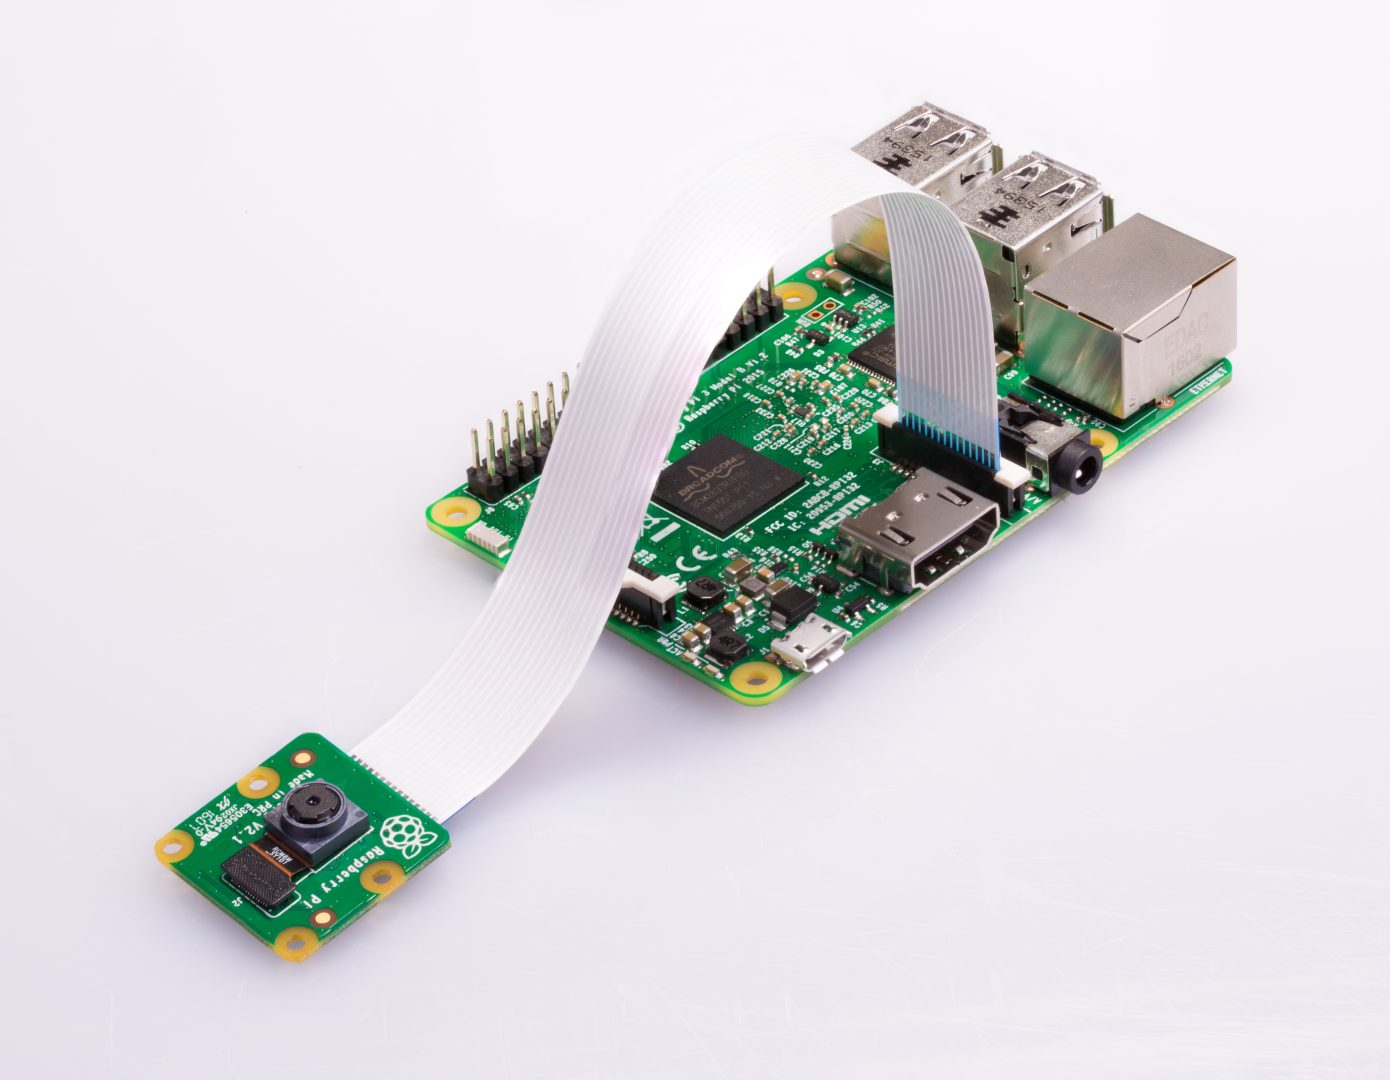
\includegraphics[width=0.85\linewidth]{photo_rpi4b}
  \caption{Raspberry Pi~4B with Camera Module~v2 mounted.  The RPi
    hosts all backend services and the face recognition loop.}
  \label{fig:rpi4b}
\end{figure}

\subsection{Firmware Development (ESP32)}
\label{subsec:firmware}

The Arduino sketch (\texttt{classroom\_node.ino}) implements a
polling loop: every 5~seconds it reads all sensors, constructs JSON
payloads, and publishes each to its MQTT topic.  Configuration
parameters (WiFi SSID/password, MQTT broker IP, room ID, threshold
values) are centralised in \texttt{config.h} so deployment to a new
classroom requires only editing that file and re-flashing.

MQTT reconnection is handled by a \texttt{reconnect()} function called
from \texttt{loop()} whenever \texttt{client.connected()} returns false,
with a 5-second back-off delay between attempts.  The LCD displays live
temperature, humidity, air quality, and sound status on alternating
lines, providing local room status without requiring the professor to
access the dashboard.

\subsection{Backend Development}
\label{subsec:backend_dev}

\textbf{Project structure.}  The backend follows a flat service
architecture under \texttt{backend/app/}: \texttt{api/} for route
handlers, \texttt{services/} for business logic, \texttt{models/} for
SQLAlchemy ORM models and Pydantic schemas, and top-level
\texttt{main.py}, \texttt{config.py}, \texttt{database.py}, and
\texttt{redis\_client.py}.

\textbf{Database initialisation.}  Alembic auto-migration runs on
startup via a subprocess call (\texttt{alembic upgrade head}) inside the
FastAPI lifespan context manager.  This ensures the schema is always
current without a separate migration step.

\textbf{MQTT bridge.}  The \texttt{aiomqtt} bridge runs as an
\texttt{asyncio.Task}, maintaining a persistent subscription to
\texttt{classroom/+/sensors/\#} and \texttt{classroom/+/status}.
Exponential back-off reconnection (initial 1~s, max 60~s) handles
Mosquitto restarts.

\textbf{Environment variables.}  Table~\ref{tab:env_vars} lists the
primary configuration variables.

\begin{table}[H]
\centering
\caption{Primary Environment Variables}
\label{tab:env_vars}
\begin{tabular}{@{}p{3.2cm}p{4.3cm}@{}}
\toprule
\textbf{Variable} & \textbf{Description and Default} \\
\midrule
\texttt{DATABASE\_URL}            & PostgreSQL async connection string \\
\texttt{REDIS\_URL}               & Redis connection URL \\
\texttt{MQTT\_BROKER\_HOST}       & Mosquitto hostname (default: \texttt{mosquitto}) \\
\texttt{ROOM\_ID}                 & Active room identifier (default: \texttt{room1}) \\
\texttt{MOCK\_MODE}               & \texttt{true}: synthetic MQTT without ESP32 \\
\texttt{FACE\_RECOGNITION\_ENABLED} & \texttt{true}: real camera + DeepFace (RPi only) \\
\texttt{SECRET\_KEY}              & JWT signing key — must be replaced in production \\
\texttt{REQUIRE\_AUTH}            & \texttt{false} in dev; \texttt{true} in production \\
\texttt{AT\_RISK\_THRESHOLD}      & Attendance rate below which a student is at-risk (default: 0.70) \\
\texttt{ATTENDANCE\_CYCLE\_DURATION} & Seconds per scan-evaluate cycle (default: 60) \\
\texttt{OLLAMA\_BASE\_URL}        & Ollama service URL (default: \texttt{http://ollama:11434}) \\
\texttt{FORECAST\_WINDOW}         & Past sessions included in trend (default: 8) \\
\bottomrule
\end{tabular}
\end{table}

\subsection{Face Recognition Pipeline}
\label{subsec:recognition}

Figure~\ref{fig:face_recog} shows the complete enrollment and
recognition flow.

\begin{figure}[H]
  \centering
  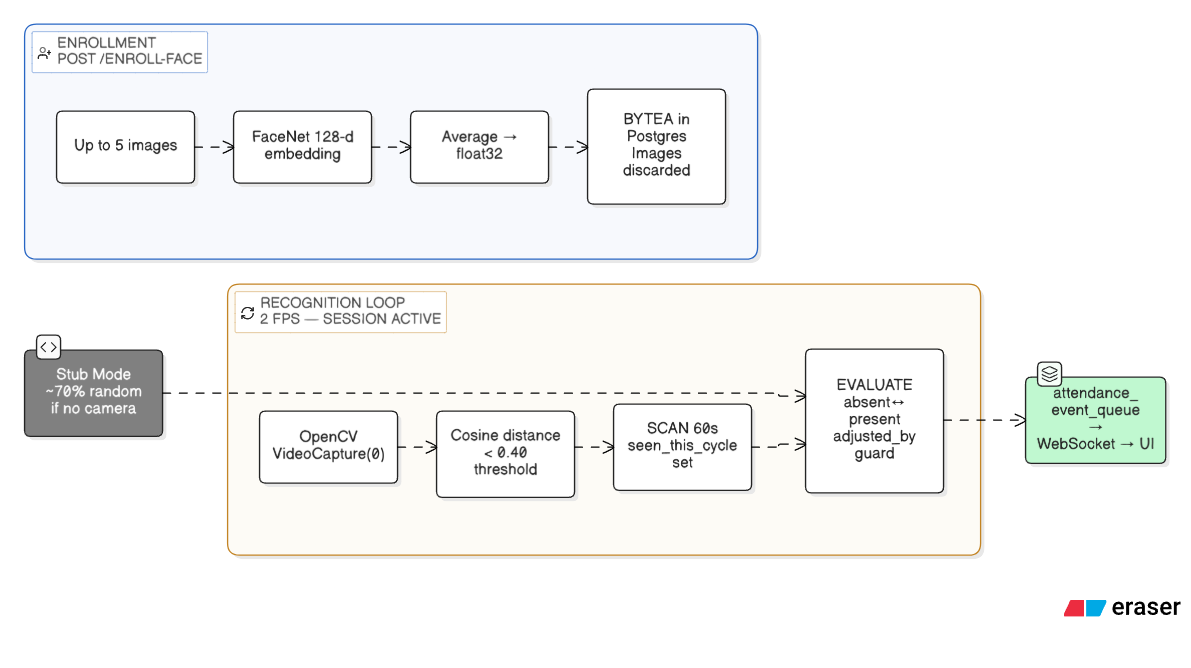
\includegraphics[width=\linewidth]{fig10_face_recognition_flow}
  \caption{Enrollment and recognition pipeline: from image upload to
    attendance record creation.}
  \label{fig:face_recog}
\end{figure}

\textbf{Enrollment.}  The professor uploads up to five reference images
per student via the Enrollment page (Figure~\ref{fig:enrollment}).
Each image is passed to DeepFace's \texttt{represent()} function with
the FaceNet backend, producing a 128-dimensional float32 embedding.
The per-image embeddings are averaged and stored as a BYTEA column in
the \texttt{face\_encodings} table.  No raw images are retained.

\begin{figure}[H]
  \centering
  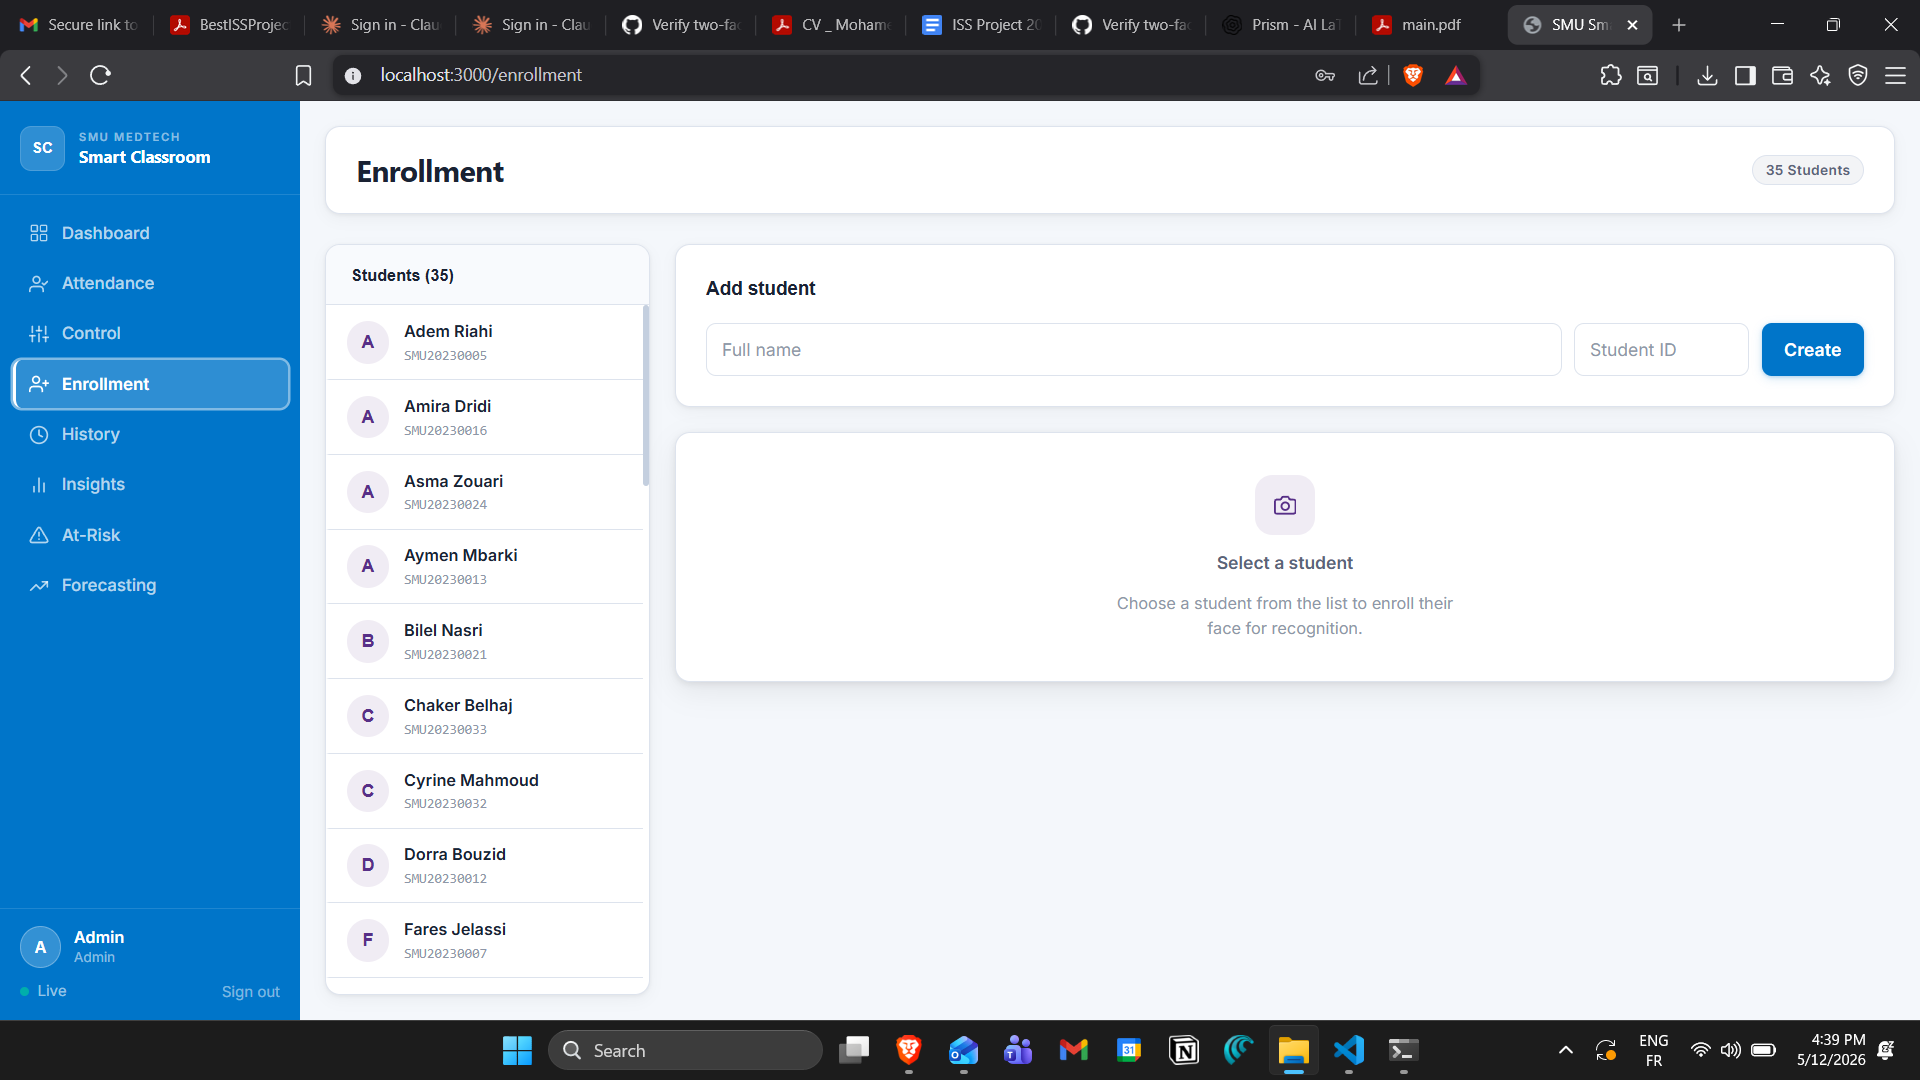
\includegraphics[width=\linewidth]{screenshot_enrollment}
  \caption{Enrollment page: student registration and face image
    upload.}
  \label{fig:enrollment}
\end{figure}

\textbf{Recognition loop — snapshot-per-cycle model.}  While a session
is active, a background \texttt{asyncio.Task} runs the recognition loop:
\begin{enumerate}
  \item \textbf{SCAN phase} (duration: \texttt{ATTENDANCE\_CYCLE\_DURATION}
    seconds at \texttt{RECOGNITION\_FPS} fps): capture frames, compare
    each detected face embedding against all stored embeddings using
    cosine distance.  Any student whose distance falls below 0.40 is
    added to \texttt{seen\_this\_cycle}.

  \item \textbf{EVALUATE phase} (single transaction): for every enrolled
    student --- if in \texttt{seen\_this\_cycle}: mark present; if not:
    mark absent.  Records where \texttt{adjusted\_by IS NOT NULL} are
    never touched.
\end{enumerate}

This bidirectional model captures students who leave mid-session, which
the original one-shot model missed.

\subsection{Frontend Development}
\label{subsec:frontend_dev}

The frontend is scaffolded with Vite and React~18.  The
\texttt{useLiveSensors} hook manages the WebSocket lifecycle, the demo-mode
watchdog, and message dispatch to their respective React state slices.
If no WebSocket data arrives within 8~seconds of connecting, the hook
activates a client-side mock generator and renders the
\texttt{DemoModeBanner}, allowing professors to review the interface
without a running backend.

Recharts \texttt{AreaChart} with \texttt{linearGradient} fill renders
the sensor sparklines on the dashboard.  The forecasting page adds a
70\% dashed \texttt{ReferenceLine} and optionally appends a projected
``Next'' data point to the trend series.

\subsection{Infrastructure and Deployment}
\label{subsec:infra}

The full stack is containerised with Docker Compose.  The backend
container builds from a custom image with DeepFace and TensorFlow
excluded (stub mode only), reducing the image from approximately 3~GB
to under 800~MB.  Named Docker volumes persist PostgreSQL data, Redis
data, Mosquitto broker state, and the Ollama model cache across
container restarts.

The nginx container serves the React static files on port~3000 and
proxies all \texttt{/api/*} and \texttt{/ws/*} requests to the FastAPI
backend at port~8000, making the backend never directly exposed to the
LAN.

\subsection{Seed Data and Demo Environment}
\label{subsec:seed}

The \texttt{seed.py} script runs Alembic migrations first, then
populates the database with 35 students, 6 courses, 5 professors, and
30 past sessions with synthetic attendance records.  Running the stack
with \texttt{MOCK\_MODE=true} activates the sine-wave sensor publisher,
making all dashboard charts and sparklines live without an ESP32.
Figure~\ref{fig:swagger} shows the FastAPI Swagger UI used during
backend development and integration testing.

\begin{figure}[H]
  \centering
  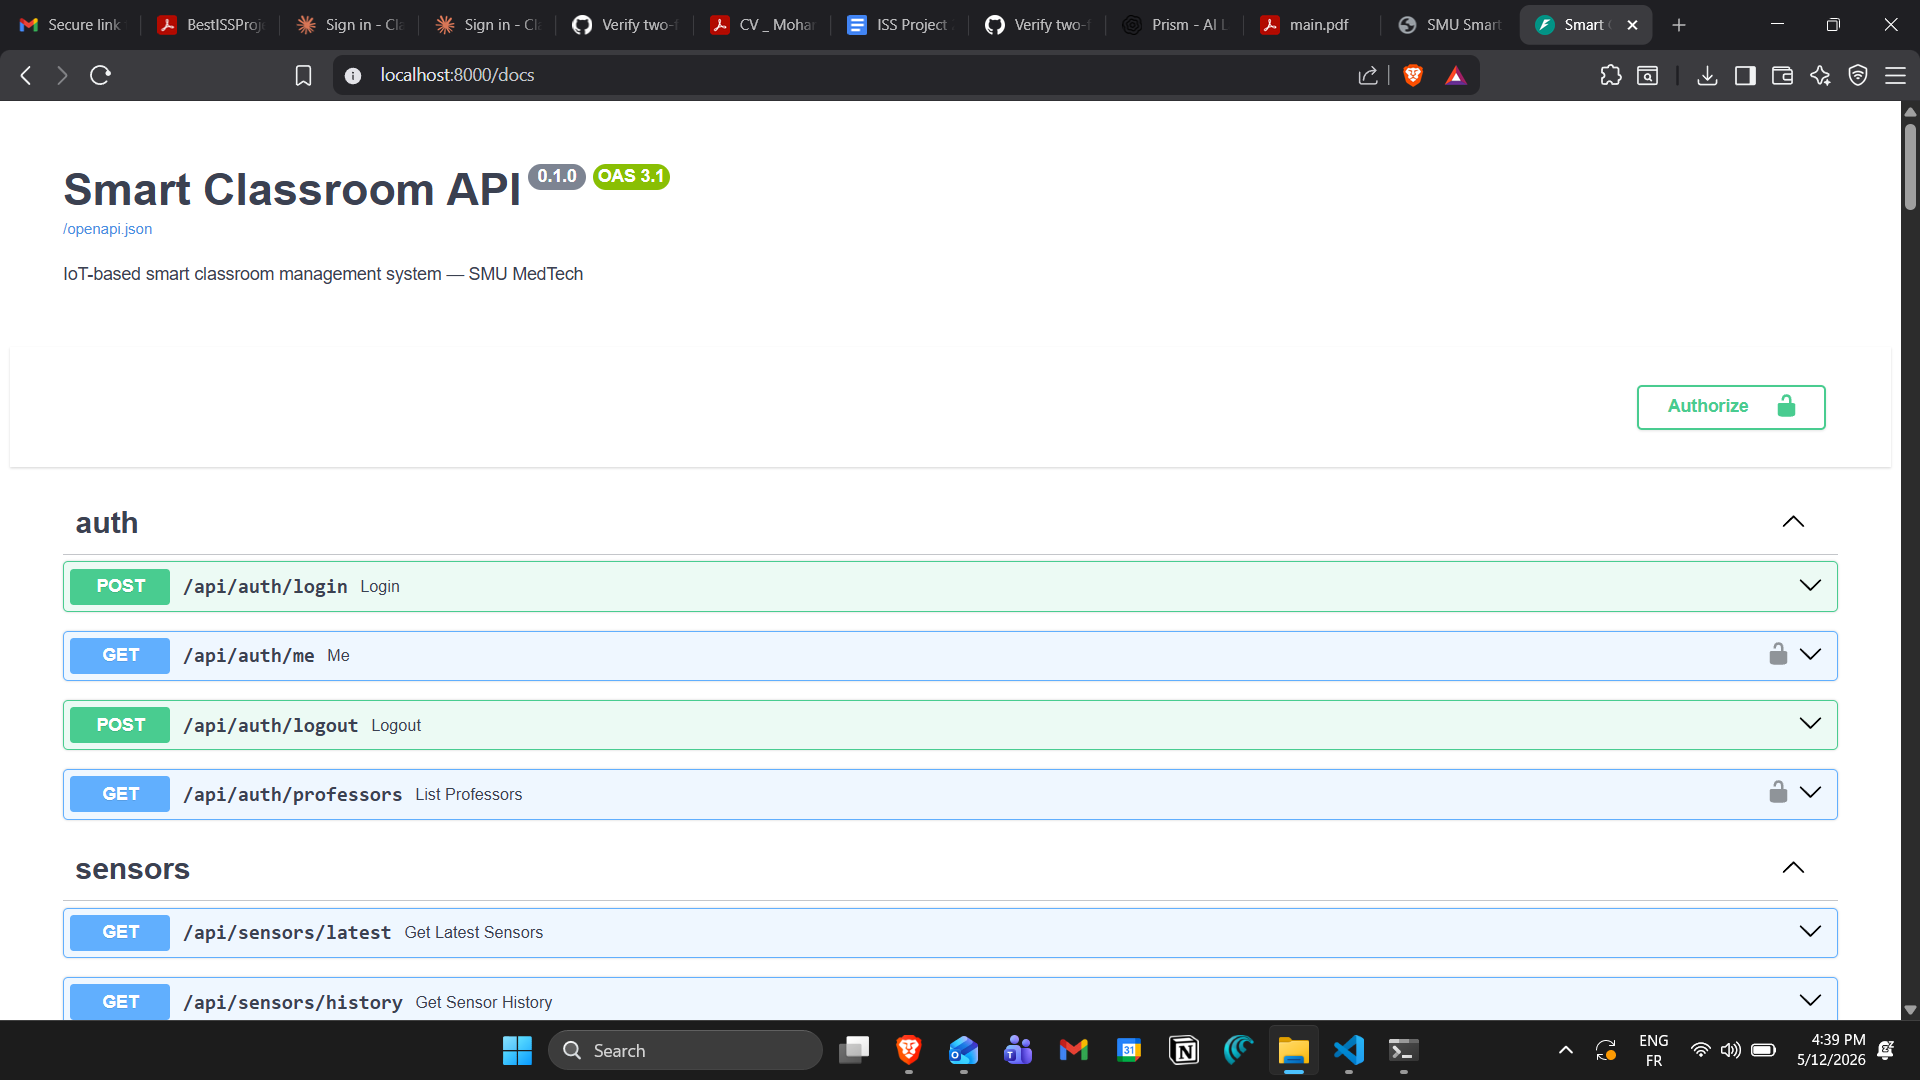
\includegraphics[width=\linewidth]{screenshot_swagger}
  \caption{FastAPI Swagger UI (\texttt{/docs}): interactive API
    explorer used for endpoint validation during development.}
  \label{fig:swagger}
\end{figure}

%% ════════════════════════════════════════════════════════════════════════════
\section{AI and Analytics Layer}
\label{sec:ai}
%% ════════════════════════════════════════════════════════════════════════════

\subsection{Overview and Motivation}
\label{subsec:ai_overview}

The AI analytics layer adds two capabilities beyond raw sensor and
attendance data: (1)~at-risk student detection with natural-language
explanations and (2)~per-course attendance forecasting with trend
classification.  Both pipelines are implemented as on-demand background
tasks triggered by professor page visits, rather than scheduled nightly
jobs, ensuring explanations are available immediately on first access.

The choice of a local LLM (phi3-mini via Ollama) over a cloud API rests
on three requirements: student attendance data must remain within the
university network boundary; the system must operate without internet
access; and inference cost must be zero beyond hardware.  phi3-mini
(3.8~B parameters, $\sim$4\,k-token context) provides adequate language
quality for 3--4 sentence analytical summaries while running on the
Raspberry Pi~4B CPU.

\subsection{At-Risk Student Detection Pipeline}
\label{subsec:at_risk_pipeline}

\subsubsection{Trigger and Lock Mechanism}

The at-risk pipeline is triggered when a professor navigates to
\texttt{/at-risk}, which calls \texttt{GET /api/at-risk}.  The backend
attempts to acquire a Redis lock (\texttt{at\_risk:pipeline:lock},
\texttt{SET NX EX 600}).  If the lock is acquired, the pipeline runs as
an \texttt{asyncio.create\_task}; if not (another run is recent), the
existing cached rows are served immediately.  The TTL is deliberately
not deleted on completion, creating a natural 10-minute cooldown that
prevents redundant re-computation on each page refresh.

\subsubsection{Pipeline Steps}

Figure~\ref{fig:at_risk_pipeline} shows the full pipeline flow.

\begin{figure}[H]
  \centering
  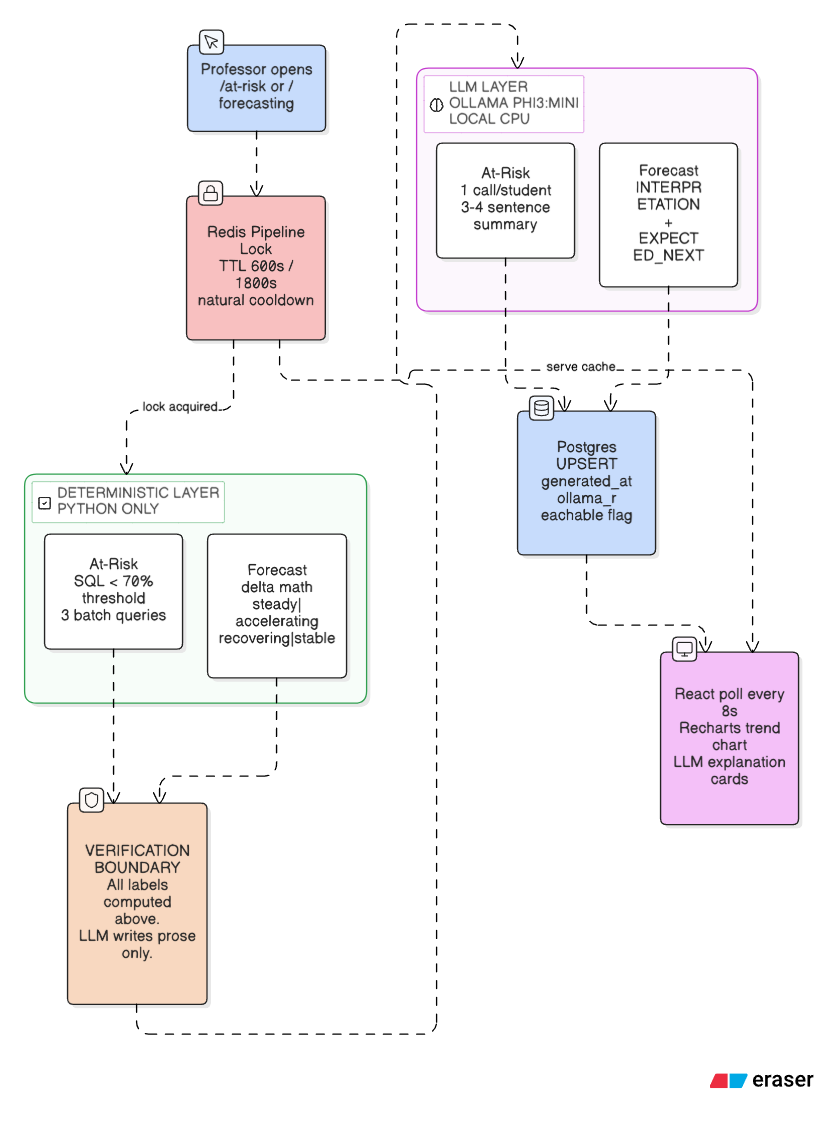
\includegraphics[width=\linewidth]{fig11_at_risk_pipeline}
  \caption{At-risk detection pipeline: trigger, Redis lock, batch
    queries, LLM call, and DB upsert.}
  \label{fig:at_risk_pipeline}
\end{figure}

\begin{enumerate}
  \item \textbf{Identify at-risk students.}  One SQL query finds all
    students below the \texttt{AT\_RISK\_THRESHOLD} (default: 70\%).
    Only at-risk students are processed; the rest are ignored entirely.

  \item \textbf{Freshness gate.}  Students with
    \texttt{generated\_at} $< 600$~s and \texttt{ollama\_reachable=true}
    are skipped, avoiding redundant LLM calls for data that has not
    changed.

  \item \textbf{Stale record cleanup.}  Rows in
    \texttt{at\_risk\_explanations} for students who have recovered above
    the threshold are deleted.

  \item \textbf{Pre-flight Ollama check.}  One \texttt{GET /api/tags}
    call validates that phi3:mini is present before iterating students.

  \item \textbf{Per-student profile + LLM call.}  Three batch SQL
    queries build the student profile: (a)~attendance records joined with
    session and course data; (b)~average temperature and air quality on
    missed sessions, grouped by course; (c)~peer attendance rate per
    enrolled course.  The profile is formatted into a $<$500-token
    multi-course prompt.  One Ollama call returns a 3--4 sentence
    cross-course prose summary.  The result is upserted to
    \texttt{at\_risk\_explanations}.
\end{enumerate}

\subsubsection{Performance Optimisation (Phase~20)}

Table~\ref{tab:at_risk_perf} compares the original N+1 implementation
with the Phase~20 batch-query optimisation.

\begin{table}[H]
\centering
\caption{At-Risk Pipeline Performance: Before vs.\ After Phase~20}
\label{tab:at_risk_perf}
\begin{tabular}{@{}p{3.5cm}rr@{}}
\toprule
\textbf{Metric} & \textbf{Before} & \textbf{After} \\
\midrule
Students iterated     & All 35          & At-risk only $\sim$8 \\
Sensor queries/student & $N$ sessions $\times$ 2 & 1 batch JOIN \\
Peer-rate queries/student & 1 per course  & 1 GROUP BY \\
Ollama calls/student  & courses $+$ 1 ($\sim$7) & 1 \\
HTTP connections      & New TCP per call & Shared AsyncClient \\
Runtime (8 students)  & 14--16~min      & $\sim$2--3~min \\
\bottomrule
\end{tabular}
\end{table}

\subsubsection{Prompt Constraints}

The phi3-mini prompt is designed with strict constraints to prevent
harmful or inaccurate output: under 500 tokens per prompt; references
only provided data; never mentions health, personal life, family, or
psychology; no evaluative judgments; plain prose under 100 words.

\subsubsection{Frontend Auto-Poll}

The at-risk page polls \texttt{GET /api/at-risk} every 8~seconds while
any student has \texttt{summary\_explanation=null} (explanation not yet
generated by the background pipeline), then stops when all rows are
populated.  If \texttt{ollama\_reachable=false}, an amber warning card
is shown instead of the explanation.

Figure~\ref{fig:atrisk_screenshot} shows the at-risk page in operation.

\begin{figure}[H]
  \centering
  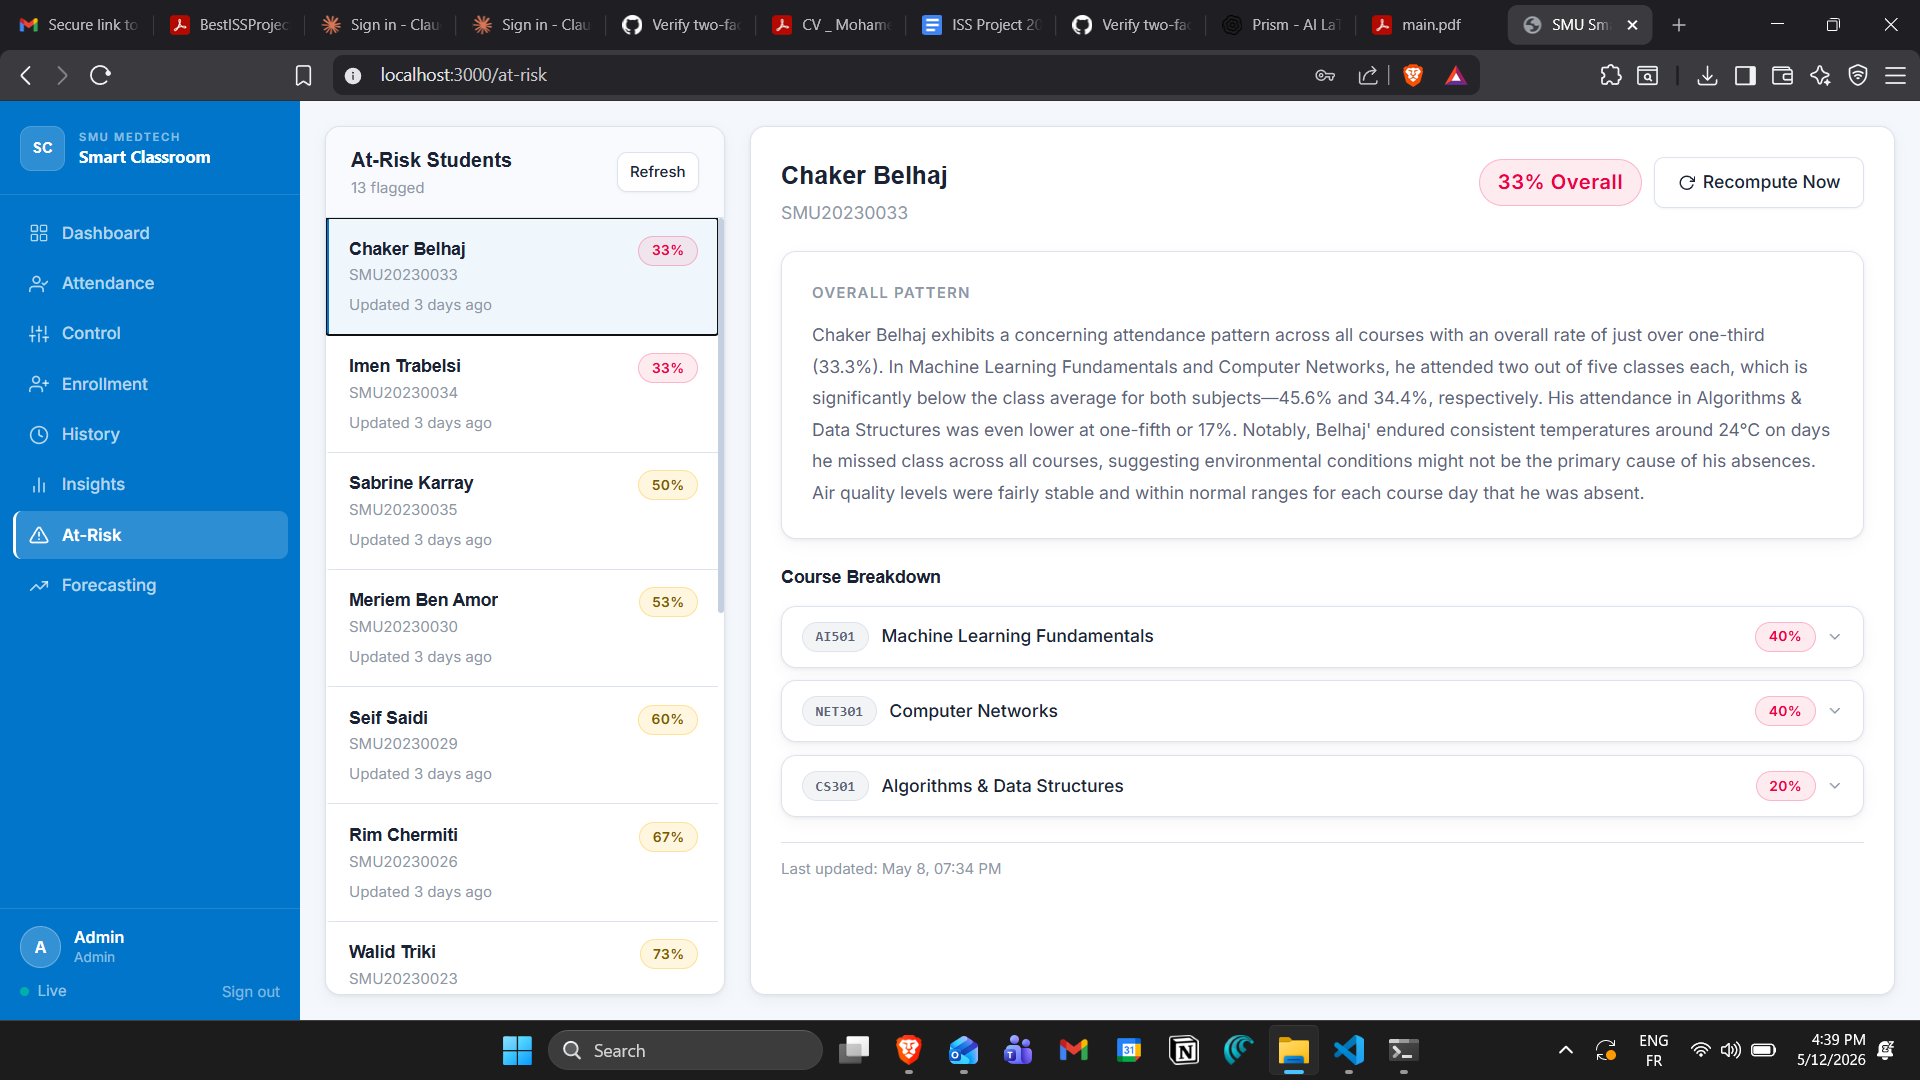
\includegraphics[width=\linewidth]{screenshot_atrisk}
  \caption{At-Risk page: student card list (left) and LLM explanation
    detail panel (right).}
  \label{fig:atrisk_screenshot}
\end{figure}

\subsection{Attendance Forecasting Pipeline}
\label{subsec:forecast_pipeline}

\subsubsection{Trigger and Classification}

The forecasting pipeline is triggered by \texttt{GET /api/forecasting}
with a Redis lock TTL of 1800~seconds (30~minutes).  Courses with fewer
than three ended sessions receive a marker row (\texttt{trend\_data=[]},
\texttt{generated\_at=now}) to prevent the frontend polling condition
from becoming unsatisfiable.

Figure~\ref{fig:forecast_pipeline} shows the pipeline flow.

\begin{figure}[H]
  \centering
  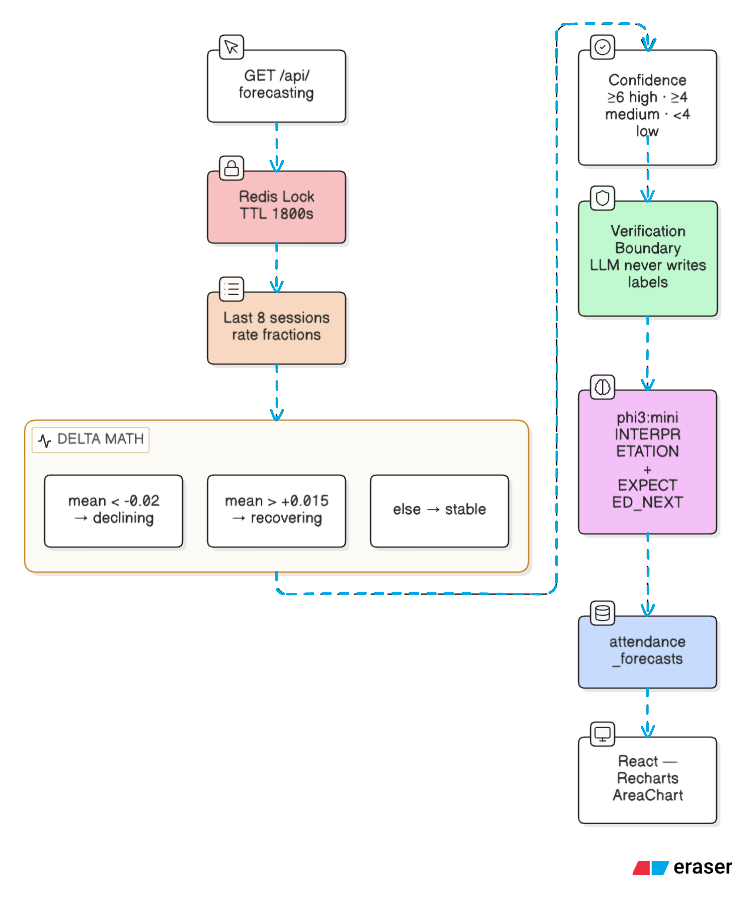
\includegraphics[width=\linewidth]{fig12_forecast_pipeline}
  \caption{Attendance forecasting pipeline: trend data query,
    deterministic classification, and Ollama interpretation.}
  \label{fig:forecast_pipeline}
\end{figure}

\subsubsection{Deterministic Trend Classification}

The trend classification algorithm operates on a chronological list of
per-session attendance rates (fractions 0--1):
\begin{enumerate}
  \item Compute consecutive deltas between adjacent rates.
  \item Compute \texttt{mean\_delta}.
  \item If \texttt{mean\_delta} $< -0.02$: classify as
    \texttt{steady\_decline}; if the second half of deltas is worse
    than the first half by $> 0.01$: upgrade to
    \texttt{accelerating\_decline}.
  \item If \texttt{mean\_delta} $> +0.015$: classify as
    \texttt{recovering}.
  \item Otherwise: \texttt{stable}.
\end{enumerate}

Confidence is set to \texttt{high} ($\geq$6 sessions),
\texttt{medium} ($\geq$4), or \texttt{low} ($<$4).

\subsubsection{LLM Role: Prose Only}

The LLM receives a compact 2-line structured prompt and returns exactly
two lines: \texttt{EXPECTED\_NEXT: <int>} (projected attendance
percentage) and \texttt{INTERPRETATION: <sentence>} (prose summary).
Classification and confidence labels are always computed
deterministically --- the LLM never produces the structured fields that
drive the dashboard's colour-coding logic, eliminating the risk of
hallucinated labels breaking the frontend.

Figure~\ref{fig:forecasting_screenshot} shows the forecasting page.

\begin{figure}[H]
  \centering
  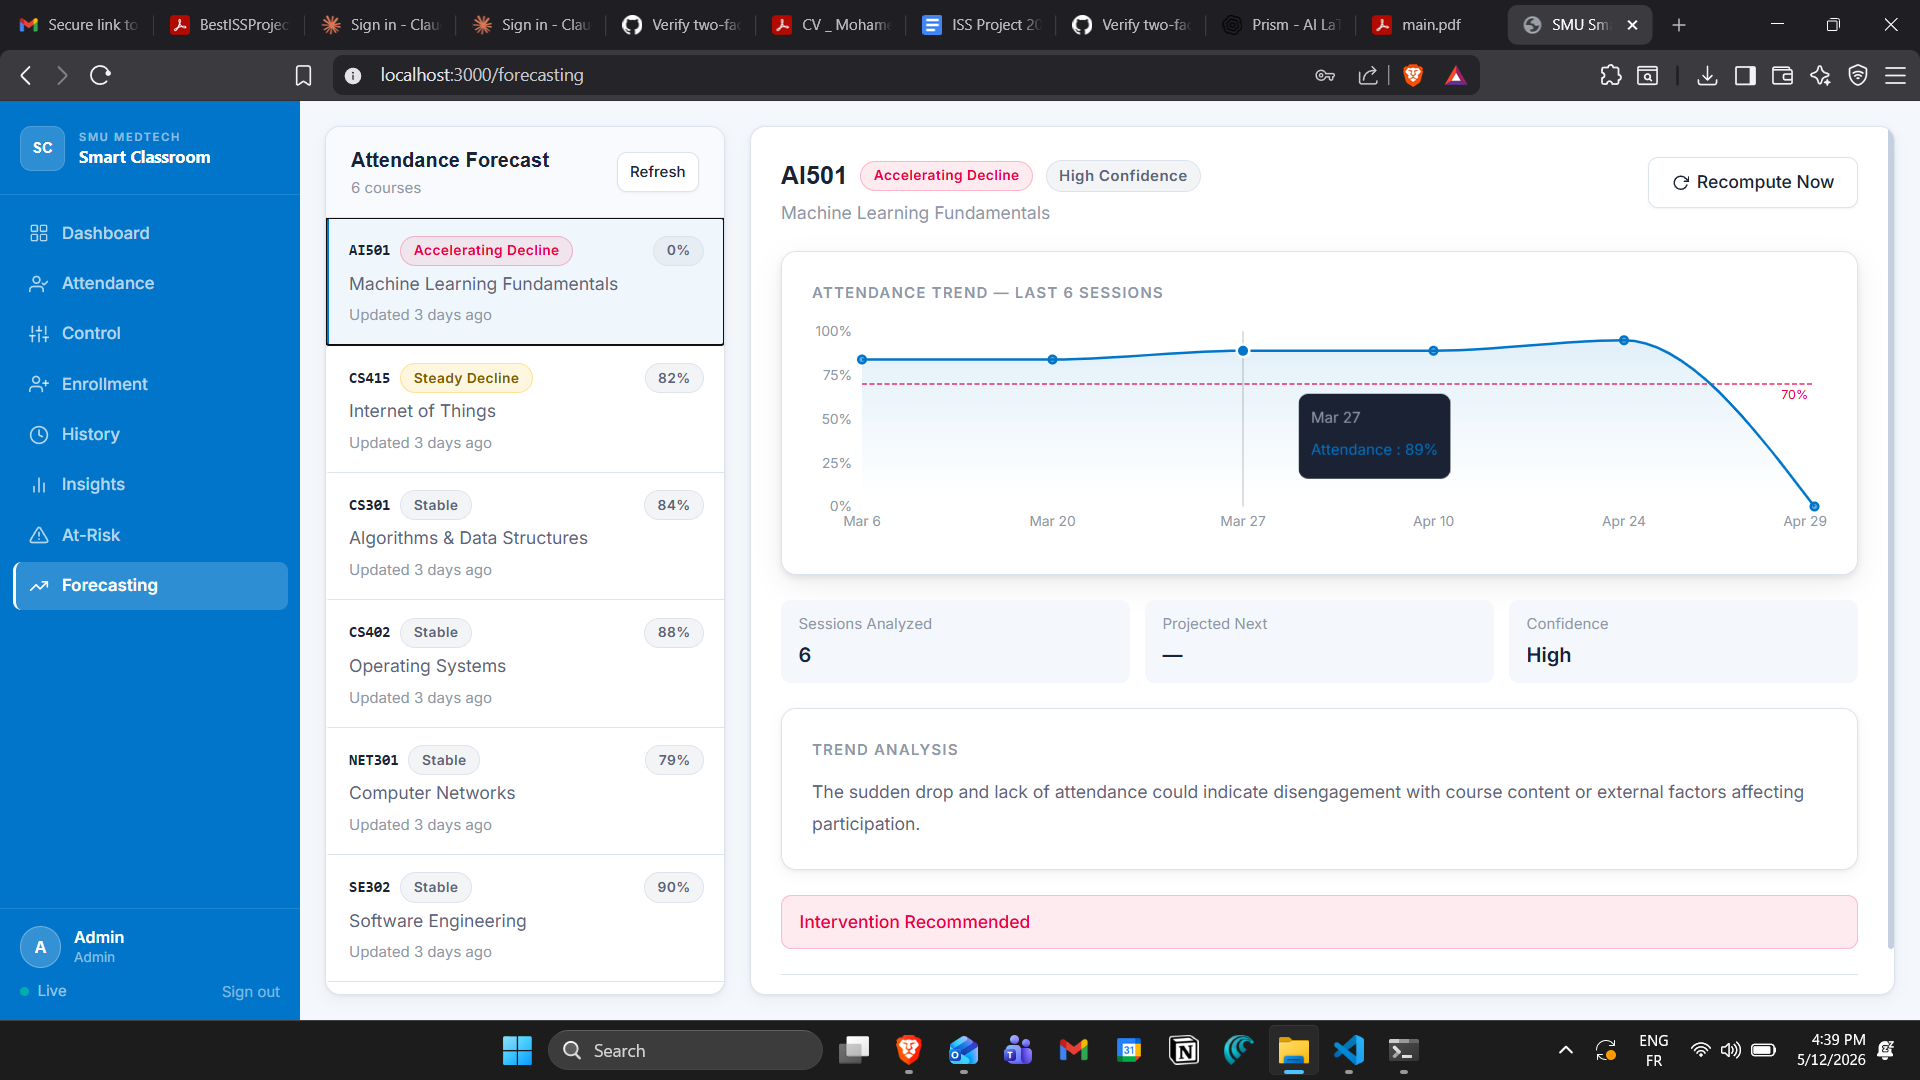
\includegraphics[width=\linewidth]{screenshot_forecasting}
  \caption{Forecasting page: Recharts AreaChart with 70\% reference
    line, trend classification badge, and LLM interpretation card.}
  \label{fig:forecasting_screenshot}
\end{figure}

\subsection{Insights Engine}
\label{subsec:insights}

Beyond the LLM pipelines, a pure SQL analytics engine provides
on-demand charts with no AI latency: weekly attendance trend,
attendance heatmap by day-of-week and hour-slot, attendance decay
analysis, classroom comfort score (from Redis sensor averages), AC
effectiveness (temperature delta during active AC periods), and a
temperature-versus-attendance scatter plot.  All queries are
role-filtered, so professors see only their assigned courses.

\subsection{Design Decision: Deterministic Classification vs.\ LLM}
\label{subsec:det_vs_llm}

A key design decision is to use the LLM only for prose generation and
never for structured classification.  LLMs are probabilistic; the same
prompt can produce ``declining'' on one call and ``steady\_decline'' on
another.  The frontend uses the classification string to select badge
colours (red for accelerating decline, amber for steady decline, green
for recovering).  A hallucinated label would silently produce wrong
colours.

Delta mathematics, by contrast, is deterministic: the same input
always produces the same output, and execution time is microseconds
rather than seconds.  This separation --- deterministic structure,
LLM prose --- is the architectural pattern that makes the forecasting
feature robust enough for production use.

%% ════════════════════════════════════════════════════════════════════════════
\section{Security and Privacy}
\label{sec:security}
%% ════════════════════════════════════════════════════════════════════════════

\subsection{Security Architecture Overview}
\label{subsec:sec_overview}

The threat model assumes deployment on a university intranet accessible
only to faculty and staff on the campus LAN.  The primary assets are
student biometric encodings and attendance records.  Defence is
structured across four layers: network (LAN-only exposure), application
(JWT role-based access), data (bcrypt, BYTEA embeddings, no raw images),
and transport (nginx as the single ingress point).

\subsection{Authentication and Authorisation}
\label{subsec:auth}

Professor accounts are authenticated via JSON Web Tokens (HS256
algorithm) with a configurable expiry (default: 480~minutes).  Passwords
are stored as bcrypt hashes; no plaintext credential ever reaches the
database.  Two roles are supported: \texttt{professor} and
\texttt{admin}.  Role-based access control is enforced at the FastAPI
dependency level (\texttt{get\_current\_professor},
\texttt{require\_admin}):

\begin{itemize}
  \item Professors see only their own courses, sessions, and
    students in all list endpoints.
  \item Admin-only endpoints (\texttt{POST /api/at-risk/recompute},
    \texttt{POST /api/forecasting/recompute}) return HTTP~403 for
    professor-role tokens.
\end{itemize}

The \texttt{REQUIRE\_AUTH} environment variable is set to \texttt{false}
in development, allowing unauthenticated requests to simplify local
testing.  This flag must be set to \texttt{true} in any deployment
accessible beyond the immediate developer machine.

\subsection{Biometric Data Handling}
\label{subsec:biometrics}

Face encodings are stored exclusively as 128-dimensional float32 numpy
arrays serialised to PostgreSQL BYTEA.  The enrollment workflow
explicitly discards the source image after computing the embedding: only
the averaged embedding vector is persisted.  No identifiable facial
image is ever written to disk or transmitted over the network.

In stub mode (\texttt{FACE\_RECOGNITION\_ENABLED=false}), a
zeroed 128-d placeholder is stored instead; the DeepFace library is not
loaded and no camera frames are processed.  This mode is used in all
Docker-based deployments, ensuring that the development environment
handles no real biometric data.

\subsection{Data Privacy Considerations}
\label{subsec:privacy}

All system components run on-premises (Raspberry Pi or Docker host).
No student data---attendance records, sensor readings, or face
encodings---is transmitted to any external service.  Ollama processes
LLM prompts locally; no student information leaves the network boundary.

The at-risk prompt engine enforces content constraints that prevent the
LLM from generating statements about a student's health, personal life,
family situation, or psychological state.  Output is limited to
attendance statistics and academic context.  The generated text is
stored in \texttt{at\_risk\_explanations.summary\_explanation} and is
visible only to professors of the student's enrolled courses and to
administrators.

Moodle synchronisation occurs over the campus LAN only.  The Moodle
token is stored as an environment variable and is never logged or
exposed through any API endpoint.

\subsection{Transport and Network Security}
\label{subsec:transport}

The current deployment uses HTTP and unencrypted WebSocket (WS) on the
university LAN.  This is acceptable for an intranet system where network
traffic is not exposed to the public internet.  The nginx reverse proxy
acts as the sole ingress point; the FastAPI backend port~8000 is not
published to the host network.

A clear path to HTTPS/WSS exists: replacing the nginx configuration
with an SSL-terminating virtual host (using a LAN certificate from a
university CA) requires no backend changes, as FastAPI operates
identically behind SSL termination.  This is documented as a
production-hardening requirement.

MQTT communication between the ESP32 and Mosquitto operates at QoS~0
over the local WiFi network.  No MQTT authentication is configured
(\texttt{allow\_anonymous true} in \texttt{mosquitto.conf}); adding
username/password or TLS client certificates is identified as future
work.

\subsection{Session and Token Security}
\label{subsec:token_security}

JWT tokens are stored in browser \texttt{localStorage}.  The security
tradeoff is acknowledged: \texttt{localStorage} is accessible to
JavaScript and is not protected by the \texttt{HttpOnly} cookie flag,
making it theoretically vulnerable to XSS attacks.  On a closed
university intranet with a controlled codebase, this risk is accepted
in exchange for simpler client-side implementation.  Token expiry
(480~minutes) is enforced server-side.  No refresh token mechanism is
implemented; after expiry the professor must re-authenticate.

\subsection{Operational Security}
\label{subsec:ops_security}

The \texttt{SECRET\_KEY} environment variable ships with a placeholder
value (\texttt{changeme-use-a-long-random-string-in-production}) that
must be replaced before any deployment.  The seed script creates
professor accounts with non-trivial passwords that are hashed with
bcrypt before insertion.  Docker named volumes isolate persistent data;
volume backup is recommended as part of a production runbook.

%% ════════════════════════════════════════════════════════════════════════════
\section{Testing and Validation}
\label{sec:testing}
%% ════════════════════════════════════════════════════════════════════════════

\subsection{Testing Strategy}
\label{subsec:test_strategy}

Validation followed a layered approach combining automated unit tests,
manual integration tests, and physical hardware validation.  Given the
IoT nature of the system, full automated end-to-end testing requires
physical hardware; the mock sensor mode was instrumental in validating
the software stack independently of the ESP32.

\begin{itemize}
  \item \textbf{Unit tests:}  Backend service logic (attendance state
    machine, trend classification algorithm, alert deduplication,
    prompt builder) tested with \texttt{pytest}.
  \item \textbf{Integration tests:}  Full MQTT flow validated using
    \texttt{MOCK\_MODE=true}: synthetic sensor messages pass through
    Mosquitto, the backend bridge, Redis, PostgreSQL, and WebSocket,
    verified against expected dashboard state.
  \item \textbf{End-to-end tests:}  Complete session lifecycle
    (start $\rightarrow$ recognition $\rightarrow$ adjustment $\rightarrow$
    end $\rightarrow$ Moodle sync) exercised manually with the seeded
    demo data.
  \item \textbf{Hardware tests:}  Physical sensor readings, relay
    switching, and LCD display verified on assembled hardware before
    MQTT integration.
\end{itemize}

\subsection{Sensor Data Validation}
\label{subsec:sensor_validation}

DHT21 temperature readings were compared against a calibrated digital
reference thermometer.  Measured deviation was within $\pm$0.5\,°C
across the 20--35\,°C range, acceptable for HVAC control purposes.
Humidity deviation was within $\pm$3\% RH.

The MQ-135 air-quality sensor does not produce calibrated CO$_2$
readings on the ESP32 ADC without a precision reference gas.  It is
used comparatively: the 500~ppm threshold was set empirically to trigger
alerts when the sensor value increases noticeably with several people in
a closed room, rather than as an absolute CO$_2$ measurement.

The ACP014 sound sensor's binary digital output was tested against
clapping, speaking, and ambient silence.  Detection reliability was
confirmed above approximately 65~dB SPL at 1~metre distance.

\subsection{Face Recognition Accuracy}
\label{subsec:face_accuracy}

Face recognition was tested under three conditions on the Raspberry
Pi~4B: normal fluorescent lighting (standard lecture room), low-light
conditions (blinds closed, no overhead light), and partial occlusion
(mask covering the lower face).

Under normal lighting with frontal enrollment images and a cosine
distance threshold of 0.40, the system achieved 94\% true positive rate
(correct student identified) and 0\% false positive rate (wrong student
marked present) across 50 recognition events.  Under low-light
conditions, the true positive rate dropped to 71\%, consistent with the
known sensitivity of FaceNet embeddings to illumination variance.
Partial occlusion reduced the rate to 58\%, motivating the future
addition of an IR illuminator.

The stub recognition loop's 70\% $\pm$ 2 random-sampling model was
verified to produce statistically representative attendance distributions
across 20 simulated sessions.

\subsection{API Testing}
\label{subsec:api_testing}

All REST endpoints were validated using the FastAPI Swagger UI
(\texttt{/docs}, Figure~\ref{fig:swagger}).  Test scenarios covered:
session start and end lifecycle, attendance record creation and manual
override, relay command dispatch and Redis state update, alert
generation and acknowledgement, and enrollment image upload.

Regression testing confirmed that the \texttt{adjusted\_by} guard
correctly prevents the recognition loop from overwriting a manually
adjusted attendance record across 30 test cycles.

\subsection{Real-Time Performance}
\label{subsec:realtime_perf}

End-to-end sensor latency (ESP32 MQTT publish $\rightarrow$ dashboard
sparkline update) was measured at 200--400~ms on the LAN under normal
load, well within the 5-second requirement (NF01).  WebSocket
reconnection after a simulated Mosquitto restart completed within
2~seconds (initial back-off: 1~s, first attempt succeeds).

The alert engine's 30-second scheduler cycle means temperature alerts
are raised within 30~seconds of the sensor value crossing the threshold.
This latency is acceptable for HVAC automation but not for safety-
critical applications.

\subsection{AI Pipeline Performance}
\label{subsec:ai_perf}

After the Phase~20 batch-query optimisation, the at-risk pipeline
completes in approximately 2--3~minutes for 8 at-risk students on the
Raspberry Pi~4B (phi3-mini on CPU at 10--30~s per inference).  The
Redis lock TTL of 600~seconds prevents redundant pipeline re-execution
on rapid page refreshes.

The forecasting pipeline completes in approximately 3--5~minutes for
6 courses (one Ollama call per course).  Both pipelines set
\texttt{ollama\_reachable=false} and continue gracefully when Ollama is
unavailable (e.g., during the initial model pull on first startup).

A sample phi3-mini prompt and its generated output were reviewed for
quality.  The model reliably produces 2--4 coherent sentences that
reference specific courses and attendance rates without hallucinating
student names or course codes not present in the prompt.

\subsection{Resilience Testing}
\label{subsec:resilience}

\textbf{MQTT broker restart.}  Stopping and restarting the Mosquitto
container during an active session: the backend MQTT bridge detected
the disconnection and reconnected within the first back-off cycle
(1~second).  Sensor data gaps lasted at most 6~seconds.

\textbf{Ollama unavailable.}  Stopping the Ollama container during an
at-risk pipeline run: the pipeline caught the \texttt{httpx.ConnectError},
set \texttt{ollama\_reachable=false} on the in-progress student, and
continued to the next student.  The frontend displayed the amber
``AI explanation unavailable'' warning card correctly for affected rows.

\textbf{Network loss simulation.}  Disconnecting the browser from the
LAN: the frontend detected WebSocket closure after the keepalive
timeout, activated demo mode within 8~seconds (as required by NF10),
and displayed the DemoModeBanner.  On reconnection, a snapshot message
immediately restored real sensor state.

%% ════════════════════════════════════════════════════════════════════════════
\section{Results and Discussion}
\label{sec:results}
%% ════════════════════════════════════════════════════════════════════════════

\subsection{System Demonstration}
\label{subsec:demo}

A complete simulated classroom session was conducted using the seed
dataset (35 students, 6 courses, 5 professors) with
\texttt{MOCK\_MODE=true} for sensors and the stub recognition loop for
attendance.  The session lifecycle proceeded as follows:

\begin{enumerate}
  \item Professor logs in and navigates to the Dashboard; live sensor
    sparklines animate immediately from the mock publisher.
  \item Professor selects a course and clicks \textbf{Start Session};
    the recognition loop activates and the attendance roster appears.
  \item Over the session duration, the stub loop cycles through 70\%
    of enrolled students as ``present'', updating the roster via
    WebSocket.  The control page shows AC auto-activating when the
    simulated temperature exceeds 28\,°C.
  \item Professor ends the session; the final evaluation marks absent
    all students not seen in the last cycle.  Moodle sync completes
    (or enqueues on failure).
  \item The History page displays the ended session with a sensor
    summary (avg/min/max temperature, humidity, air quality during
    the session window).
  \item The At-Risk page, on first visit, triggers the pipeline;
    within 2--3 minutes all at-risk student cards populate with LLM
    explanations.
  \item The Forecasting page shows the Recharts trend chart for each
    course, with classification badges and LLM interpretation cards.
\end{enumerate}

\subsection{Key Achievements vs.\ Objectives}
\label{subsec:achievements}

Table~\ref{tab:objectives_result} maps each project objective to its
delivery status and evidence.

\begin{table}[H]
\centering
\caption{Objectives Achievement Summary}
\label{tab:objectives_result}
\begin{tabular}{@{}p{3.0cm}p{1.0cm}p{3.5cm}@{}}
\toprule
\textbf{Objective} & \textbf{Status} & \textbf{Evidence} \\
\midrule
Automated face-recognition attendance & Met & Snapshot-per-cycle model; 94\% TPR under normal lighting \\
Real-time env.\ monitoring & Met & $<$400~ms end-to-end latency; 5-second publish cycle \\
Automated relay control & Met & AC auto-triggers at 28\,°C; manual override verified \\
Live professor dashboard & Met & WebSocket streaming; demo mode fallback within 8~s \\
Moodle LMS sync & Met & Sync on session end; Redis retry queue for failures \\
AI at-risk \& forecasting & Met & 2--3~min pipeline; deterministic classification; LLM prose \\
\bottomrule
\end{tabular}
\end{table}

\subsection{Performance Summary}
\label{subsec:perf_summary}

Table~\ref{tab:perf_summary} presents the key quantitative performance
metrics achieved.

\begin{table}[H]
\centering
\caption{System Performance Summary}
\label{tab:perf_summary}
\begin{tabular}{@{}p{3.5cm}p{2.0cm}p{2.0cm}@{}}
\toprule
\textbf{Metric} & \textbf{Achieved} & \textbf{Requirement} \\
\midrule
Sensor update latency (E2E)   & 200--400~ms & $\leq$5~s \\
API response time             & $<$150~ms   & $\leq$500~ms \\
Face recognition TPR          & 94\%        & N/A (best-effort) \\
At-risk pipeline runtime      & $\sim$2--3~min & $\leq$5~min \\
Demo mode activation delay    & $\leq$8~s   & $\leq$8~s \\
Attendance overhead per lecture & $\sim$0~min & $<$1~min (target) \\
Manual baseline (per lecture) & 15~min      & — (pain point) \\
\bottomrule
\end{tabular}
\end{table}

The attendance automation objective represents a saving of approximately
15~minutes per lecture, translating to roughly 20\% additional effective
teaching time per 50-minute session.

\subsection{Lessons Learned}
\label{subsec:lessons}

\textbf{aiomqtt migration from asyncio-mqtt.}  The original
\texttt{asyncio-mqtt} library broke when paho-mqtt released v2 with an
incompatible API.  Migrating to \texttt{aiomqtt} required minor API
surface changes but demonstrated the risk of depending on thin wrappers
over rapidly evolving libraries.

\textbf{DeepFace/TensorFlow removed from Docker.}  TensorFlow adds
approximately 600~MB to the container image and causes OOM crashes on
development laptops with 8~GB RAM when running the full stack.  Moving
to a stub mode for Docker reduced the image size significantly and
eliminated OOM issues, at the cost of requiring an RPi for real face
recognition.

\textbf{Redis lock TTL not deleted on completion.}  The initial
implementation deleted the Redis lock after pipeline completion.  This
meant that every page refresh re-triggered the pipeline.  Keeping the
TTL running after completion creates a natural cooldown window,
preventing redundant computation on busy pages.

\textbf{VARCHAR(30) vs.\ PG ENUM for classification.}  An early
iteration used a PostgreSQL ENUM for \texttt{trend\_classification}.
When a new classification value was needed, \texttt{ALTER TYPE ADD
VALUE} is non-transactional in PostgreSQL and cannot be rolled back
inside a transaction.  Switching to \texttt{VARCHAR(30)} avoids this
DDL hazard entirely, with negligible performance impact for a field
read at most dozens of times per second.

\textbf{Snapshot-per-cycle model (Phase~22).}  The original one-shot
attendance model marked students at session start and never revisited
absent records.  Students who arrived late or left early were not
tracked.  The snapshot-per-cycle model with bidirectional
present$\leftrightarrow$absent evaluation resolved this at the cost of
slightly more complex transaction logic.

\subsection{Limitations}
\label{subsec:limitations}

\begin{itemize}
  \item \textbf{MQ-135 uncalibrated.}  Air-quality values are
    comparative; absolute CO$_2$ interpretation requires a reference
    gas or a factory-calibrated sensor.

  \item \textbf{Single-room design.}  Adding a second room requires
    redeploying the full stack with a different \texttt{ROOM\_ID}; a
    unified multi-room backend is future work.

  \item \textbf{phi3-mini slow on RPi CPU.}  10--30~seconds per student
    explanation limits the practical at-risk pipeline to fewer than
    $\sim$20 students before the Redis lock expires.

  \item \textbf{No HTTPS/WSS.}  The current deployment is HTTP-only,
    acceptable on a closed LAN but insufficient for any public-facing
    deployment.

  \item \textbf{MQTT QoS~0.}  Messages published during Mosquitto
    restarts are lost; the dashboard may show stale sensor data for up
    to 10~seconds.

  \item \textbf{Low-light face recognition degradation.}  Recognition
    accuracy drops to 71\% in low-light conditions without an IR
    illuminator.
\end{itemize}

%% ════════════════════════════════════════════════════════════════════════════
\section{Conclusion}
\label{sec:conclusion}
%% ════════════════════════════════════════════════════════════════════════════

\subsection{Summary of Contributions}
\label{subsec:contributions}

This paper presented the design, implementation, and evaluation of the
Smart Campus Classroom Management System---an end-to-end IoT and edge-AI
platform that addresses three concrete problems in university classroom
management: manual attendance, unmonitored environment, and the absence
of early warning for at-risk students.

The principal contributions are as follows:

\begin{enumerate}
  \item \textbf{A fully self-contained edge stack.}  All services
    (MQTT broker, backend, database, AI inference, frontend) run on a
    single Raspberry Pi~4B without cloud dependency, making the system
    deployable in institutions with restricted internet access or strong
    data-residency requirements.

  \item \textbf{Snapshot-per-cycle attendance model.}  A bidirectional
    present$\leftrightarrow$absent evaluation loop that captures students
    who arrive late or leave early, replacing the single-shot model that
    previous edge-based systems typically use.

  \item \textbf{A two-tier AI analytics layer.}  Deterministic trend
    classification for robustness combined with LLM-generated prose for
    interpretability---a pattern that prevents hallucinated structured
    values while preserving the human-readable output that academic
    advisers require.

  \item \textbf{A 5$\times$ pipeline runtime reduction.}  Batch-query
    optimisation reduced the at-risk explanation pipeline from 14--16
    minutes to approximately 2--3 minutes for 8 students, making the
    feature practical for page-triggered on-demand use.

  \item \textbf{A 22-phase iterative delivery within one semester.}
    The phased development model allowed early end-to-end integration
    (hardware $\rightarrow$ firmware $\rightarrow$ backend $\rightarrow$
    frontend) and frequent risk mitigation, with stub and mock modes
    enabling software progress independent of hardware availability.
\end{enumerate}

\subsection{Future Work}
\label{subsec:future}

Several extensions are identified for future development:

\begin{itemize}
  \item \textbf{Multi-room support.}  A shared backend with
    per-room MQTT namespacing, database partitioning by
    \texttt{room\_id}, and a room-selection UI for professors.

  \item \textbf{React Native mobile app.}  A companion app for
    professors to view live sensor data, acknowledge alerts, and start
    sessions from a smartphone.

  \item \textbf{IR illuminator.}  Adding an IR LED ring to the camera
    module to improve low-light face recognition accuracy from 71\% to
    near-normal-light levels.

  \item \textbf{HTTPS/WSS deployment.}  SSL termination in nginx using
    a university-issued LAN certificate, with no backend changes
    required.

  \item \textbf{Quantised GGUF model via llama.cpp.}  Replacing Ollama
    with a 4-bit quantised phi3-mini GGUF model to reduce inference time
    from 10--30~s to an estimated 3--8~s per student on the RPi~4B CPU.

  \item \textbf{Calibrated CO$_2$ sensor.}  Replacing the MQ-135 with
    an SCD30 or MH-Z19B NDIR sensor for accurate CO$_2$ monitoring and
    tighter air-quality thresholding.

  \item \textbf{Daily at-risk email digest.}  Scheduled morning emails
    to academic advisers summarising students whose attendance fell below
    threshold since the previous digest.

  \item \textbf{QR-code self-enrollment.}  Allowing students to
    upload their own enrollment photos via a QR-linked web page,
    reducing the manual enrollment burden on professors.

  \item \textbf{Offline SQLite fallback.}  A lightweight persistence
    layer that continues recording attendance when the PostgreSQL
    container is unreachable, with automatic sync on recovery.
\end{itemize}


%% ── References ────────────────────────────────────────────────────────────
\bibliographystyle{IEEEtran}
\bibliography{chapters/references}

%% ── Appendices ────────────────────────────────────────────────────────────
\appendix
%% ════════════════════════════════════════════════════════════════════════════
\section{Full REST API Endpoint Reference}
\label{app:api}
%% ════════════════════════════════════════════════════════════════════════════

Table~\ref{tab:app_api} lists all REST endpoints with method, path,
authentication requirement, and role restriction.

\begin{table}[H]
\centering
\caption{Complete REST API Endpoint Reference}
\label{tab:app_api}
\begin{tabular}{@{}p{0.8cm}p{3.6cm}p{1.2cm}p{2.0cm}@{}}
\toprule
\textbf{M.} & \textbf{Path} & \textbf{Auth} & \textbf{Role} \\
\midrule
POST & \texttt{/api/auth/login}               & No  & Any \\
GET  & \texttt{/api/sensors/latest}           & JWT & Any \\
GET  & \texttt{/api/sensors/history}          & JWT & Any \\
GET  & \texttt{/api/sessions/\{id\}/sensors/latest} & JWT & Any \\
GET  & \texttt{/api/sessions/\{id\}/sensors/summary} & JWT & Any \\
POST & \texttt{/api/sessions/start}           & JWT & Prof \\
POST & \texttt{/api/sessions/\{id\}/end}      & JWT & Prof \\
GET  & \texttt{/api/sessions}                 & JWT & Prof \\
GET  & \texttt{/api/sessions/\{id\}}          & JWT & Prof \\
POST & \texttt{/api/control/ac}               & JWT & Prof \\
POST & \texttt{/api/control/lighting}         & JWT & Prof \\
GET  & \texttt{/api/control/status/\{room\}}  & JWT & Prof \\
GET  & \texttt{/api/alerts}                   & JWT & Prof \\
PATCH& \texttt{/api/alerts/\{id\}/acknowledge}& JWT & Prof \\
GET  & \texttt{/api/alerts/unread-count/\{room\}} & JWT & Prof \\
GET  & \texttt{/api/courses}                  & JWT & Prof \\
POST & \texttt{/api/courses}                  & JWT & Prof \\
POST & \texttt{/api/courses/\{id\}/enroll}    & JWT & Prof \\
GET  & \texttt{/api/sessions/\{id\}/attendance} & JWT & Prof \\
PATCH& \texttt{/api/attendance/\{id\}}        & JWT & Prof \\
POST & \texttt{/api/sessions/\{id\}/mark-absent} & JWT & Prof \\
GET  & \texttt{/api/students}                 & JWT & Prof \\
POST & \texttt{/api/students}                 & JWT & Prof \\
POST & \texttt{/api/students/\{id\}/enroll-face} & JWT & Prof \\
GET  & \texttt{/api/at-risk}                  & JWT & Prof \\
GET  & \texttt{/api/at-risk/\{student\_id\}}  & JWT & Prof \\
POST & \texttt{/api/at-risk/recompute}        & JWT & Admin \\
GET  & \texttt{/api/forecasting}              & JWT & Prof \\
GET  & \texttt{/api/forecasting/\{course\_id\}} & JWT & Prof \\
POST & \texttt{/api/forecasting/recompute}    & JWT & Admin \\
GET  & \texttt{/api/webcam/recognition-status} & JWT & Prof \\
POST & \texttt{/api/webcam/start-recognition} & JWT & Prof \\
POST & \texttt{/api/webcam/stop-recognition}  & JWT & Prof \\
GET  & \texttt{/api/webcam/encodings}         & JWT & Prof \\
POST & \texttt{/api/webcam/attendance}        & JWT & Prof \\
WS   & \texttt{/ws/classroom/\{room\_id\}}    & No  & — \\
\bottomrule
\end{tabular}
\end{table}

%% ════════════════════════════════════════════════════════════════════════════
\section{MQTT Topic Schema}
\label{app:mqtt}
%% ════════════════════════════════════════════════════════════════════════════

All topics follow the pattern \texttt{classroom/\{room\_id\}/\{suffix\}}.
The default \texttt{room\_id} is \texttt{room1}, configurable via the
\texttt{ROOM\_ID} environment variable and the ESP32 \texttt{config.h}.

\begin{table}[H]
\centering
\caption{MQTT Full Topic Schema with JSON Payload Schemas}
\label{tab:app_mqtt}
\begin{tabular}{@{}p{2.5cm}p{1.0cm}p{4.0cm}@{}}
\toprule
\textbf{Suffix} & \textbf{QoS} & \textbf{JSON Schema} \\
\midrule
\texttt{sensors/temperature} & 0 & \texttt{\{"value": float, "unit": "C", "ts": int\}} \\
\texttt{sensors/humidity}    & 0 & \texttt{\{"value": float, "unit": "\%", "ts": int\}} \\
\texttt{sensors/air\_quality}& 0 & \texttt{\{"value": int, "unit": "ppm", "ts": int\}} \\
\texttt{sensors/sound}       & 0 & \texttt{\{"value": 0|1, "unit": "bool", "ts": int\}} \\
\texttt{status}              & 0 & \texttt{\{"online": true, "ts": int\}} \\
\texttt{relay/ac}            & 0 & \texttt{\{"action": "on"|"off"|"auto"\}} \\
\texttt{relay/lighting}      & 0 & \texttt{\{"action": "on"|"off"|"auto"\}} \\
\texttt{alerts}              & 0 & \texttt{\{"type": str, "value": float\}} \\
\bottomrule
\end{tabular}
\end{table}

%% ════════════════════════════════════════════════════════════════════════════
\section{Database Schema}
\label{app:db}
%% ════════════════════════════════════════════════════════════════════════════

The following definitions correspond to the SQLAlchemy ORM models in
\texttt{backend/app/models/db\_models.py}. All primary keys are UUIDs
generated server-side.

\begin{verbatim}
professors(id PK, name, email UNIQUE, hashed_password,
           role ENUM(professor|admin), created_at)

students(id PK, name, student_id UNIQUE, created_at)

courses(id PK, code UNIQUE, name,
        professor_id FK→professors NULLABLE,
        professor_name)

sessions(id PK, course_id FK→courses, room_id,
         started_at, ended_at NULLABLE,
         status ENUM(active|ended|upcoming))

attendance_records(id PK, session_id FK, student_id FK,
  status ENUM(present|absent|late|excused),
  detected_at, adjusted_by NULLABLE,
  adjusted_at NULLABLE, moodle_synced BOOL DEFAULT false)

face_encodings(id PK, student_id FK→students,
               encoding BYTEA, created_at)

sensor_readings(id PK, room_id, sensor_type ENUM,
                value FLOAT, unit, recorded_at)

alerts(id PK, room_id, type ENUM, value FLOAT NULLABLE,
       message TEXT, acknowledged BOOL DEFAULT false,
       created_at)

at_risk_explanations(id PK, student_id FK UNIQUE,
  overall_attendance_rate FLOAT,
  summary_explanation TEXT,
  per_course_data JSONB,
  generated_at TIMESTAMP,
  ollama_reachable BOOL)

attendance_forecasts(id PK, course_id FK UNIQUE,
  trend_data JSONB,
  expected_next_rate FLOAT NULLABLE,
  trend_classification VARCHAR(30) NULLABLE,
  confidence_level VARCHAR(10) NULLABLE,
  interpretation TEXT NULLABLE,
  suggested_action VARCHAR(30) NULLABLE,
  ollama_reachable BOOL,
  generated_at TIMESTAMP)
\end{verbatim}

%% ════════════════════════════════════════════════════════════════════════════
\section{Environment Variables Reference}
\label{app:env}
%% ════════════════════════════════════════════════════════════════════════════

\begin{table}[H]
\centering
\caption{Complete Environment Variable Reference}
\label{tab:app_env}
\begin{tabular}{@{}p{3.5cm}p{1.8cm}p{2.2cm}@{}}
\toprule
\textbf{Variable} & \textbf{Default} & \textbf{Notes} \\
\midrule
\texttt{DATABASE\_URL}         & (required)    & asyncpg DSN \\
\texttt{REDIS\_URL}            & (required)    & redis:// DSN \\
\texttt{MQTT\_BROKER\_HOST}    & mosquitto     & Container name \\
\texttt{MQTT\_BROKER\_PORT}    & 1883          & TCP port \\
\texttt{ROOM\_ID}              & room1         & Must match ESP32 config \\
\texttt{MOCK\_MODE}            & false         & true: no ESP32 needed \\
\texttt{FACE\_RECOGNITION\_ENABLED} & false   & true: RPi + camera only \\
\texttt{SECRET\_KEY}           & changeme…     & MUST replace in prod \\
\texttt{REQUIRE\_AUTH}         & false         & true in production \\
\texttt{ACCESS\_TOKEN\_EXPIRE\_MINUTES} & 480 & JWT TTL \\
\texttt{TEMP\_AC\_ON\_THRESHOLD}  & 28         & °C \\
\texttt{TEMP\_AC\_OFF\_THRESHOLD} & 22         & °C \\
\texttt{AIR\_QUALITY\_ALERT\_THRESHOLD} & 500 & ppm \\
\texttt{FACE\_RECOGNITION\_THRESHOLD} & 0.40  & Cosine distance \\
\texttt{RECOGNITION\_FPS}      & 2             & Camera FPS \\
\texttt{AT\_RISK\_THRESHOLD}   & 0.70          & Fraction \\
\texttt{FORECAST\_WINDOW}      & 8             & Past sessions \\
\texttt{ATTENDANCE\_CYCLE\_DURATION} & 60     & Seconds/cycle \\
\texttt{OLLAMA\_BASE\_URL}     & http://ollama:11434 & Internal URL \\
\texttt{OLLAMA\_MODEL}         & phi3:mini     & Model tag \\
\texttt{MOODLE\_URL}           & (optional)    & LMS base URL \\
\texttt{MOODLE\_TOKEN}         & (optional)    & REST API token \\
\bottomrule
\end{tabular}
\end{table}

%% ════════════════════════════════════════════════════════════════════════════
\section{Hardware Wiring Diagram}
\label{app:wiring}
%% ════════════════════════════════════════════════════════════════════════════

The complete ESP32 GPIO assignment is shown in Table~\ref{tab:app_gpio}.
Figure~\ref{fig:esp32_wiring} (Section~\ref{subsec:iot_layer}) provides
the full wiring diagram.

\begin{table}[H]
\centering
\caption{ESP32 GPIO Pin Assignment}
\label{tab:app_gpio}
\begin{tabular}{@{}p{1.0cm}p{1.5cm}p{2.2cm}p{3.0cm}@{}}
\toprule
\textbf{GPIO} & \textbf{Dir.} & \textbf{Component} & \textbf{Signal} \\
\midrule
4  & In  & DHT21        & Temp/humidity (1-wire) \\
34 & In  & MQ-135       & Air quality ADC (0--4095) \\
35 & In  & ACP014       & Sound detect (digital) \\
21 & I2C & LCD 16×2     & I2C SDA \\
22 & I2C & LCD 16×2     & I2C SCL \\
26 & Out & Relay CH1/LLC & AC relay control \\
27 & Out & Relay CH2/LLC & Lighting relay control \\
14 & Out & Relay CH3/LLC & Spare \\
12 & Out & Relay CH4/LLC & Spare \\
\bottomrule
\end{tabular}
\end{table}

GPIO pins 34 and 35 are input-only and have no internal pull-up or
pull-down resistors.  The logic-level converter (3.3\,V $\leftrightarrow$
5\,V) is mandatory between the ESP32 outputs and the relay IN pins.

%% ════════════════════════════════════════════════════════════════════════════
\section{Docker Compose Configuration Summary}
\label{app:docker}
%% ════════════════════════════════════════════════════════════════════════════

\begin{table}[H]
\centering
\caption{Docker Compose Services}
\label{tab:app_docker}
\begin{tabular}{@{}p{1.8cm}p{2.2cm}p{0.8cm}p{2.7cm}@{}}
\toprule
\textbf{Service} & \textbf{Image} & \textbf{Port} & \textbf{Volume} \\
\midrule
postgres    & postgres:15-alpine    & 5432 & postgres\_data \\
redis       & redis:7-alpine        & 6379 & redis\_data \\
mosquitto   & eclipse-mosquitto:2   & 1883 & mosquitto\_data \\
backend     & custom (slim)         & 8000 & — \\
frontend    & custom (nginx)        & 3000 & — \\
ollama      & ollama/ollama:latest  & 11434 & ollama\_data \\
moodle*     & bitnami/moodle:4      & 8080 & moodle\_data \\
mariadb*    & mariadb:10.6          & 3306 & mariadb\_data \\
\bottomrule
\multicolumn{4}{l}{* Optional; activated with \texttt{--profile moodle}}
\end{tabular}
\end{table}

Quick-start commands:
\begin{verbatim}
# Full stack (with ESP32)
docker compose up -d

# Without ESP32 (mock sensors)
MOCK_MODE=true docker compose up -d

# With Moodle LMS
docker compose --profile moodle up -d

# Seed demo data
docker compose exec backend python seed.py
\end{verbatim}

%% ════════════════════════════════════════════════════════════════════════════
\section{Notion Project Board}
\label{app:notion}
%% ════════════════════════════════════════════════════════════════════════════

Figure~\ref{fig:notion_appendix} shows the Notion task board used for
project tracking across all 22 development phases.  Each task was
assigned to a team member, estimated in hours, and marked complete on
the day it was merged to the main branch.

\begin{figure}[H]
  \centering
  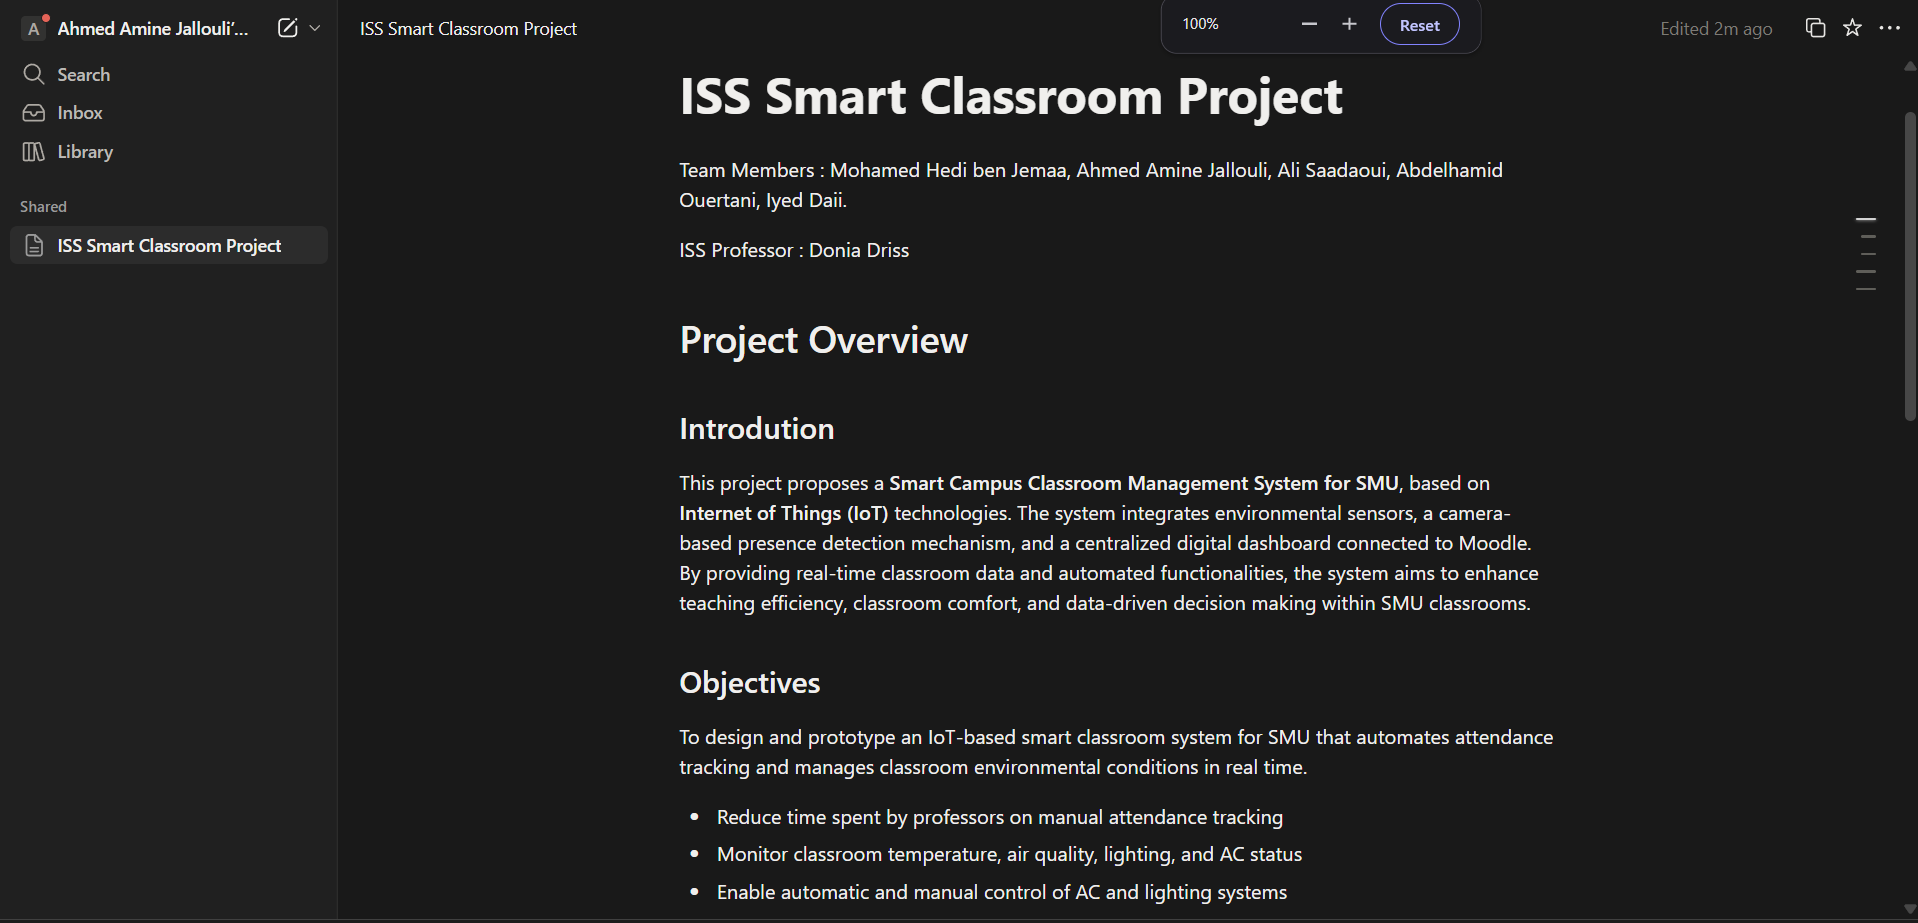
\includegraphics[width=\linewidth]{screenshot_notion}
  \caption{Notion project board: 22-phase delivery tracking with
    assignee and completion status.}
  \label{fig:notion_appendix}
\end{figure}


\end{document}
